
\section{AVL-B\"aume}
Es gibt verschiedene Varianten von geordneten bin\"aren B\"aumen, bei denen auch im
schlechtesten Fall die Anzahl der Vergleiche nur logarithmisch von der Zahl der Schl\"ussel
abh\"angt.  Eine solche Variante sind die \emph{AVL-B\"aume} \cite{adelson:62}, die nach ihren Erfindern
G.~M.~Adel'son-Vel'ski\u{\i} und E.~M.~Landis benannt sind.  Diese Variante stellen wir jetzt vor.
Dazu definieren wir zun\"achst die \emph{H\"ohe} eines bin\"aren Baums:
\begin{enumerate}
\item $\textsl{nil}.\textsl{height}() = 0$.
\item $\textsl{node}(k,v,l,r).\textsl{height}() = 1 + \max\bigl( l.\textsl{height}(), r.\textsl{height}() \bigr)$.
\end{enumerate}

\begin{Definition}[AVL-Baum] \hspace*{\fill} \\
{\em 
  Wir definieren die Menge $\AVL$ der \emph{AVL-B\"aume} induktiv:
  \begin{enumerate}
  \item $\textsl{nil} \in \AVL$.
  \item $\textsl{node}(k,v,l,r) \in \AVL$ \quad g.d.w. 
        \begin{enumerate}
        \item $\textsl{node}(k,v,l,r) \in \Bin_<$,
        \item $l, r \in \AVL$ \quad und
        \item $|l.\textsl{height}() - r.\textsl{height}()| \leq 1$.

              Diese Bedingungen bezeichnen wir auch als die \emph{Balancierungs-Bedingung}.
        \end{enumerate}
        AVL-B\"aume sind also geordnete bin\"are B\"aume, f\"ur die sich an jedem Knoten
        $\textsl{node}(k,v,l,r)$ die H\"ohen der Teilb\"aume $l$ und $r$ maximal um 1
        unterscheiden.  \hspace*{\fill} $\Box$
  \end{enumerate}
}  
\end{Definition}


Um  AVL-B\"aume zu  implementieren, k\"onnen wir auf unserer Implementierung der geordneten
bin\"aren B\"aume aufsetzen. 
Neben den Methoden, die wir schon aus der Klasse \textsl{Map} kennen, brauchen wir noch
die Methode \\[0.2cm]
\hspace*{1.3cm} $\textsl{restore}: \Bin_< \rightarrow \AVL$, \\[0.2cm]
mit der wir die Bedingung \"uber den H\"ohenunterschied von
Teilb\"aumen wiederherstellen k\"onnen, wenn diese beim Einf\"ugen oder L\"oschen eines Elements
verletzt wird.  
Der Aufruf $b.\textsl{restore}()$ setzt voraus, dass $b$ ein geordneter bin\"arer Baum ist,
f\"ur den au{\ss}er an der Wurzel \"uberall die Balancierungs-Bedingung erf\"ullt ist.
An der Wurzel kann die H\"ohe des linken Teilbaums um maximal 2 von der H\"ohe des rechten
Teilbaums abweichen. Beim Aufruf der Methode $b.\textsl{restore}()$ liegt also einer der
beiden folgenden F\"alle vor: 
\begin{enumerate}
\item $b = \textsl{nil}$ \quad oder
\item $b = \textsl{node}(k,v,l,r) \wedge l \in \AVL \wedge r \in \AVL \wedge
       |l.\textsl{height}() - r.\textsl{height}()| \leq 2$.
\end{enumerate}
 Wir spezifizieren die Methode $\textsl{restore}()$ durch
bedingte Gleichungen.
\begin{enumerate}
\item $\textsl{nil}.\textsl{restore}() = \textsl{nil}$,

      denn der leere Baum ist ein AVL-Baum.
\item $|l.\textsl{height}() - r.\textsl{height}()| \leq 1 \rightarrow \textsl{node}(k,v,l,r).\textsl{restore}() = \textsl{node}(k,v,l,r)$,

      denn wenn die Balancierungs-Bedingung bereits erf\"ullt ist,
      braucht nichts getan werden.
\item $\begin{array}[t]{cl}
              & l_1.\textsl{height}() = r_1.\textsl{height}() + 2    \\ 
       \wedge & l_1 = \textsl{node}(k_2,v_2,l_2,r_2)               \\
       \wedge & l_2.\textsl{height}() \geq r_2.\textsl{height}()     \\[0.2cm]
       \rightarrow & \textsl{node}(k_1,v_1,l_1,r_1).\textsl{restore}() = 
                     \textsl{node}\bigl(k_2,v_2,l_2,\textsl{node}(k_1,v_1,r_2,r_1)\bigr)
       \end{array}
      $

      Um diese Gleichung zu verstehen, betrachten wir Abbildung \ref{fig:casell}
      auf Seite \pageref{fig:casell}.  Der linke Teil der Abbildung beschreibt die
      Situation vor dem Ausbalancieren, es wird also der Baum \\[0.2cm]
      \hspace*{1.3cm} $\textsl{node}(k_1,v_1, \textsl{node}(k_2,v_2,l_2,r_2), r_1)$ \\[0.2cm]
      dargestellt.  Der rechte Teil der Abbildung zeigt das Ergebnis des
      Ausbalancierens, es wird also der Baum \\[0.2cm]
      \hspace*{1.3cm} $\textsl{node}\bigl(k_2,v_2,l_2,\textsl{node}(k_1,v_1,r_2,r_1)\bigr)$ \\[0.2cm]
      dargestellt. Wir haben hier die H\"ohen der einzelnen Teilb\"aume jeweils in die
      zweiten Zeilen der entsprechenden Markierungen geschrieben.  Hier ist $h$ die H\"ohe
      des Teilbaums $l_2$. Der Teilbaum $r_1$ hat die H\"ohe $h - 1$.  Der Teilbaum $r_2$
      hat die H\"ohe $h'$ und es gilt $h' \leq h$. Da $r_2$ ein AVL-Baum ist, gilt also
      entweder $h' = h$ oder $h' = h-1$.

      Die gezeigte Situation kann entstehen,
      wenn im linken Teilbaum $l_2$ ein Element eingef\"ugt wird oder wenn im rechten
      Teilbaum $r_1$ eine Element gel\"oscht wird.

      \begin{figure}[!ht]
        \centering
        \framebox{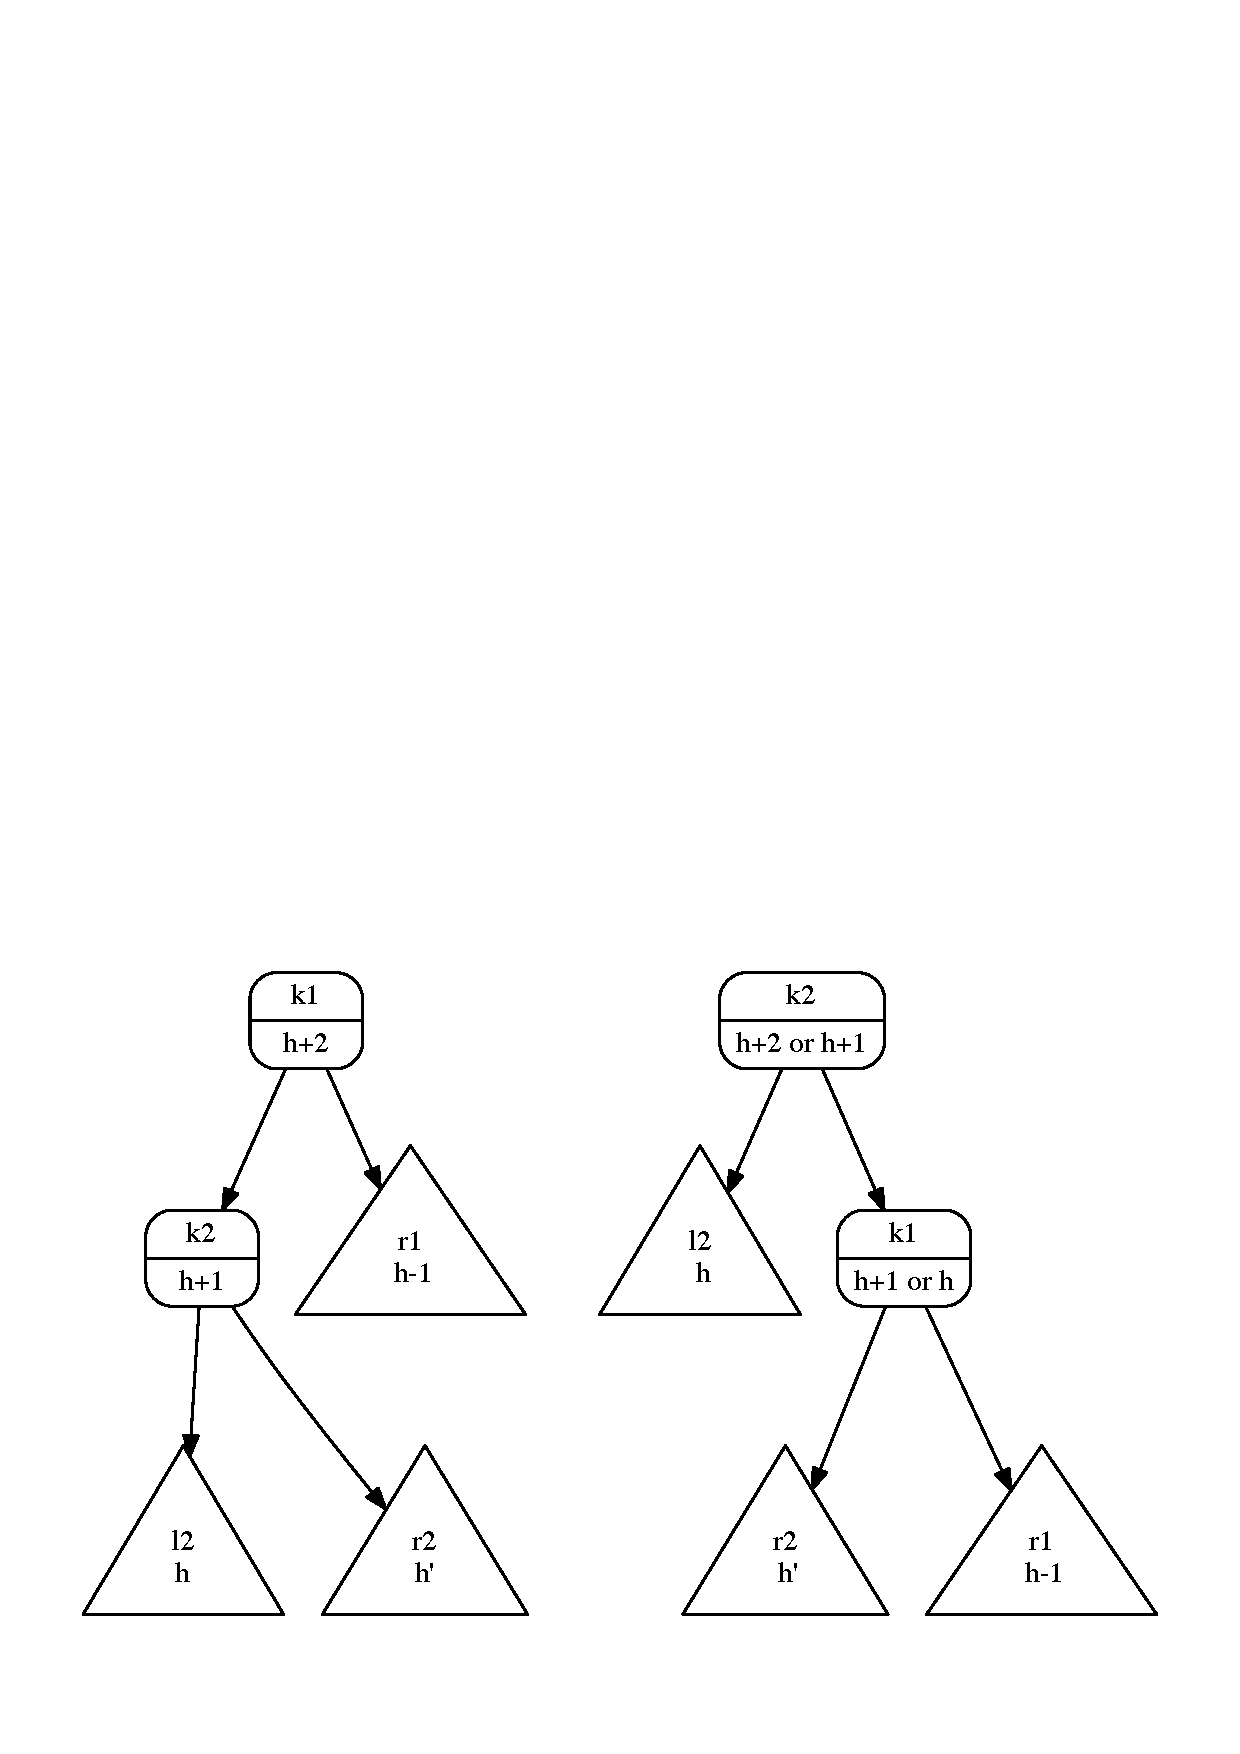
\epsfig{file=casell,scale=0.7}} 
        \caption{Ein unbalancierter Baum und der rebalancierte Baum}
        \label{fig:casell}
      \end{figure}

      Wir m\"ussen uns davon \"uberzeugen, dass der im rechten Teil von Abbildung
      \ref{fig:casell} gezeigte Baum auch tats\"achlich ein AVL-Baum ist.   Was die
      Balancierungs-Bedingung angeht, so rechnet man dies sofort nach.  Die Tatsache,
      dass der mit $k_1$ markierte Knoten entweder die H\"ohe $h$ oder $h+1$ hat folgt
      daraus, dass $r_1$ die H\"ohe $h-1$ hat und dass $h' \in \{h, h-1\}$ gilt.

      Um zu sehen, dass
      der Baum geordnet ist, k\"onnen wir  folgende Ungleichung hinschreiben: \\[0.2cm]
      \hspace*{1.3cm} $l_2 < k_2 < r_2 < k_1 < r_1$. \hspace*{\fill} $(\star)$\\[0.2cm]
      Dabei  schreiben wir f\"ur einen Schl\"ussel $k$ und einen Baum $b$ \\[0.2cm]
      \hspace*{1.3cm} $k < b$ \\[0.2cm]
      um auzudr\"ucken, dass $k$ kleiner ist als alle Schl\"ussel, die in dem Baum $b$ vorkommen.
      Analog schreiben wir $b < k$ wenn alle Schl\"ussel, die in dem Baum $b$ vorkommen,
      kleiner sind als der Schl\"ussel $k$.  Die Ungleichung $(\star)$ beschreibt die Anordnung
      der Schl\"ussel sowohl f\"ur den im linken Teil der Abbildung gezeigten Baum als auch
      f\"ur den Baum im rechten Teil der Abbildung und damit sind beide B\"aume geordnet.
\item $\begin{array}[t]{cl}
               & l_1.\textsl{height}() = r_1.\textsl{height}() + 2    \\ 
        \wedge & l_1 = \textsl{node}(k_2,v_2,l_2,r_2)               \\
        \wedge & l_2.\textsl{height}() < r_2.\textsl{height}()     \\
        \wedge & r_2 = \textsl{node}(k_3,v_3,l_3,r_3)               \\
        \rightarrow & \textsl{node}(k_1,v_1,l_1,r_1).\textsl{restore}() = 
                      \textsl{node}\bigl(k_3,v_3,\textsl{node}(k_2,v_2,l_2,l_3),\textsl{node}(k_1,v_1,r_3,r_1) \bigr)
        \end{array}
       $

        Die linke Seite der  Gleichung wird durch die Abbildung \ref{fig:caselr} auf Seite
        \pageref{fig:caselr}
        illustriert.  Dieser Baum kann in der Form \\[0.2cm]
        \hspace*{1.3cm} 
        $\textsl{node}\bigl(k_1,v_1,\textsl{node}(k_2,v_2,l_2,\textsl{node}\bigl(k_3,v_3,l_3,r_3)\bigr),r_1\bigr)$ \\[0.2cm]
        geschrieben werden. Die Teilb\"aume $l_3$ und $r_3$ haben hier entweder die H\"ohe $h$ oder
        $h-1$, wobei mindestens einer der beiden Teilb\"aume die H\"ohe $h$ haben muss.
\begin{figure}[!ht]
  \centering
  \framebox{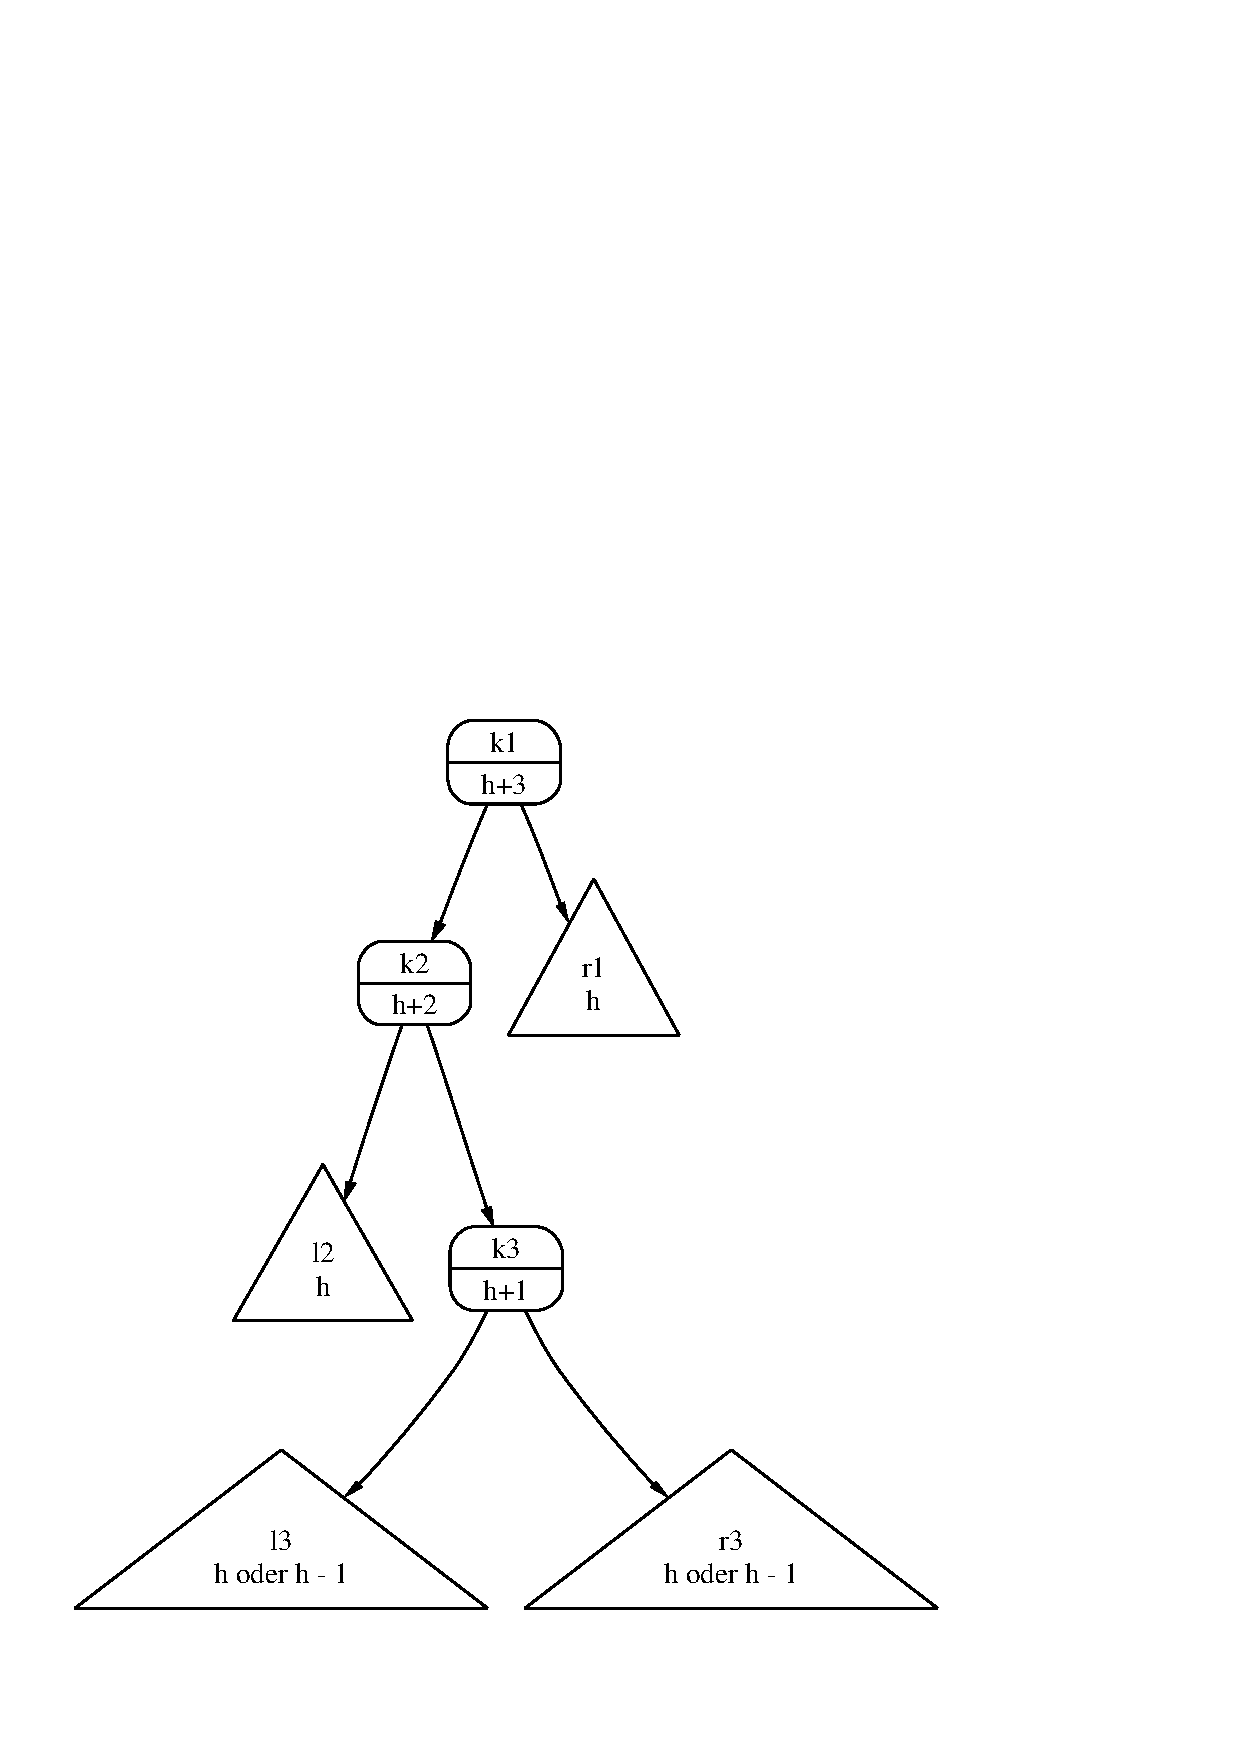
\epsfig{file=caselr,scale=0.7}} 
  \caption{Ein unbalancierter Baum: 2. Fall}
  \label{fig:caselr}
\end{figure}

     Die Situation der rechten Seite der obigen Gleichung zeigt Abbildung
     \ref{fig:caselr-nach} auf Seite \pageref{fig:caselr-nach}.  Der auf dieser
     Abbildung gezeigte Baum hat die Form \\[0.2cm]
     \hspace*{1.3cm} 
     $\textsl{node}\bigl(k_3,v_3,\textsl{node}(k_2,v_2,l_2,l_3),\textsl{node}(k_1,v_1,r_3,r_1) \bigr)$.


\begin{figure}[!ht]
  \centering
  \framebox{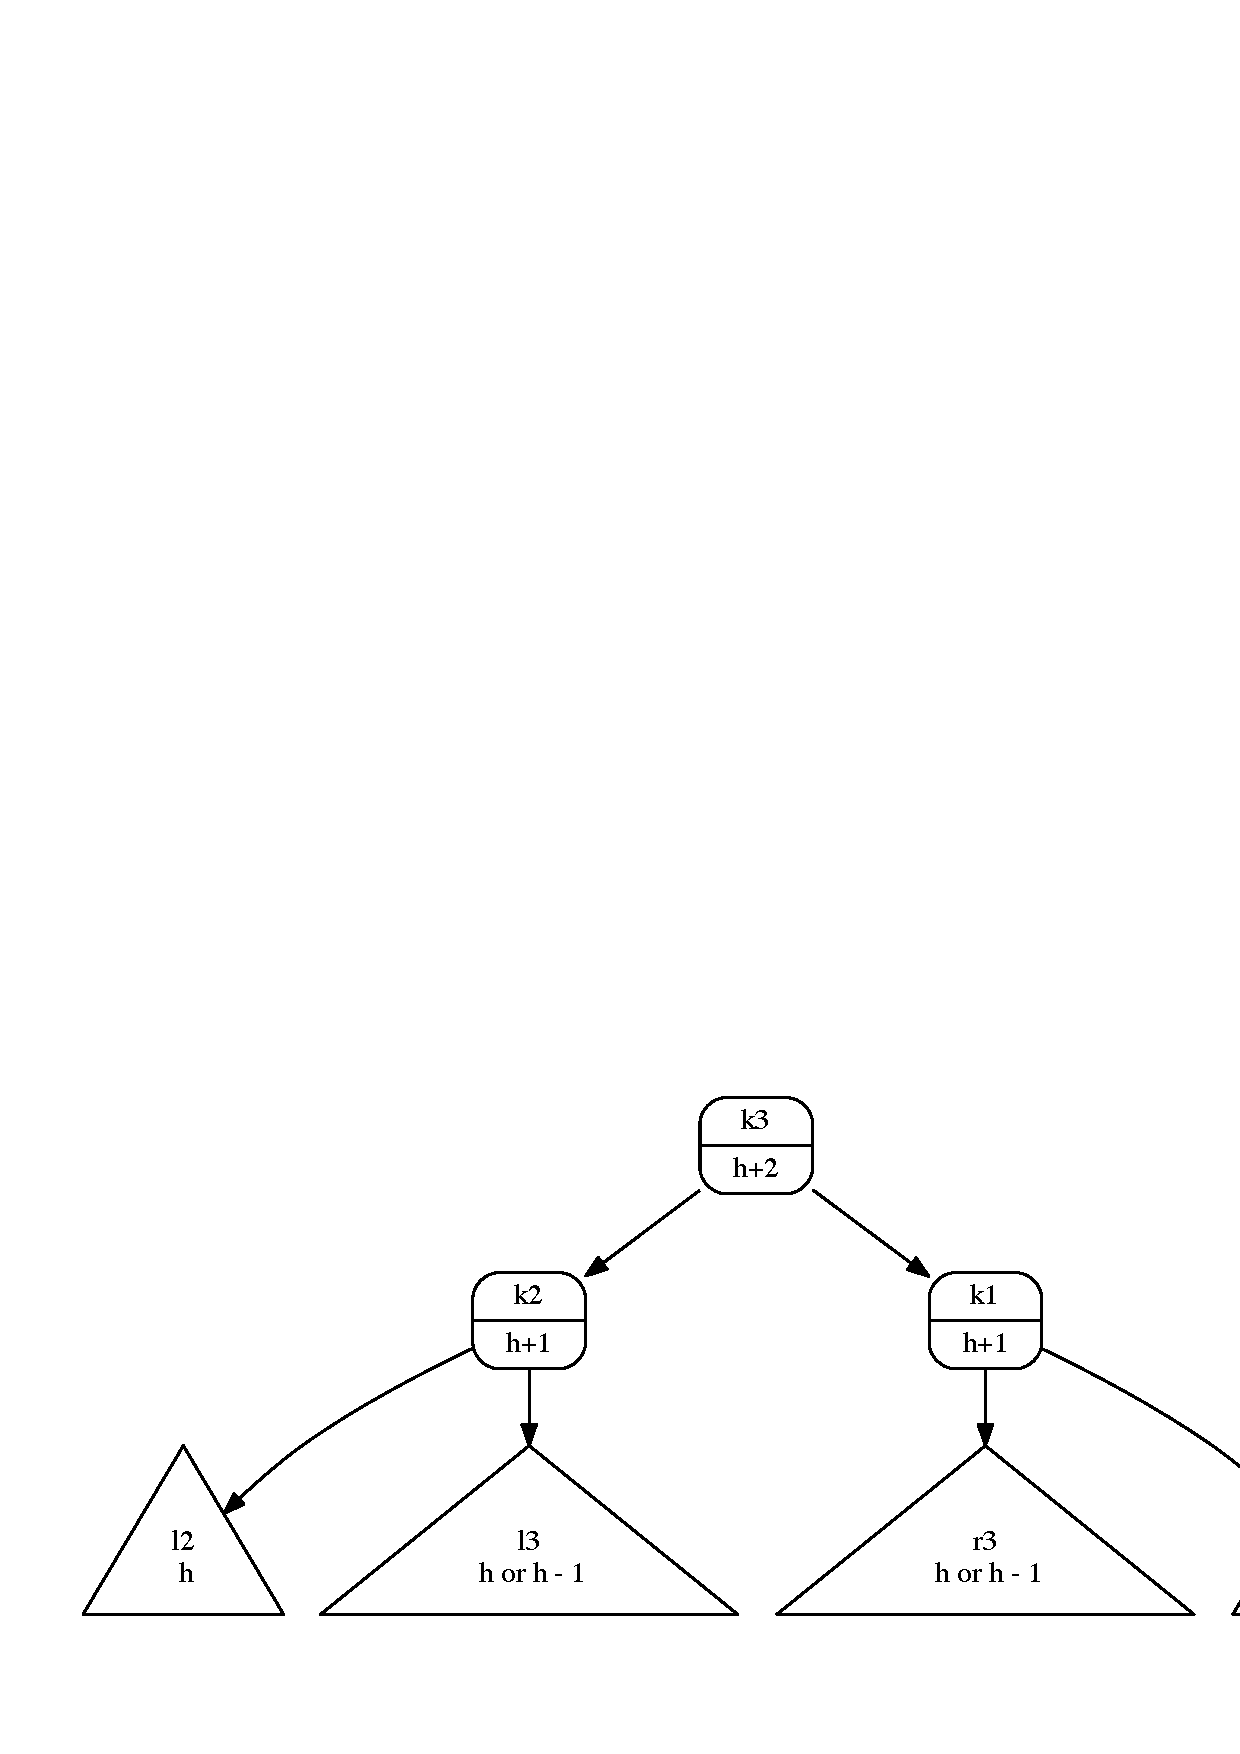
\epsfig{file=caselr-nach,scale=0.7}} 
  \caption{Der rebalancierte Baum im 2. Fall}
  \label{fig:caselr-nach}1
\end{figure}

      Die Ungleichung, die die Anordnung der Schl\"ussel sowohl im linken als auch rechten
      Baum wieder gibt, lautet\\[0.2cm]
      \hspace*{1.3cm} $l_2 < k_2 < l_3 < k_3 < r_3 < k_1 < r_1$.

      Es gibt noch zwei weitere F\"alle die auftreten, wenn der rechte Teilbaum um mehr als
      Eins gr\"o{\ss}er ist als der linke Teilbaum.  Diese beiden F\"alle sind aber zu den beiden
      vorherigen F\"allen v\"ollig analog, so dass wir die Gleichungen hier ohne weitere
      Diskussion angeben.
\item $\begin{array}[t]{cl}
              & r_1.\textsl{height}() = l_1.\textsl{height}() + 2    \\ 
       \wedge & r_1 = \textsl{node}(k_2,v_2,l_2,r_2)               \\
       \wedge & r_2.\textsl{height}() \geq l_2.\textsl{height}()     \\[0.2cm]
       \rightarrow & \textsl{node}(k_1,v_1,l_1,r_1).\textsl{restore}() = 
                     \textsl{node}\bigl(k_2,v_2,\textsl{node}(k_1,v_1,l_1,l_2),r_2\bigr)
       \end{array}
      $
\item $\begin{array}[t]{cl}
               & r_1.\textsl{height}() = l_1.\textsl{height}() + 2    \\ 
        \wedge & r_1 = \textsl{node}(k_2,v_2,l_2,r_2)               \\
        \wedge & r_2.\textsl{height}() < l_2.\textsl{height}()     \\
        \wedge & l_2 = \textsl{node}(k_3,v_3,l_3,r_3)               \\
        \rightarrow & \textsl{node}(k_1,v_1,l_1,r_1).\textsl{restore}() = 
                      \textsl{node}\bigl(k_3,v_3,\textsl{node}(k_1,v_1,l_1,l_3),\textsl{node}(k_2,v_2,r_3,r_2) \bigr)
        \end{array}
       $

\end{enumerate}
Damit k\"onnen wir nun die Methode $\textsl{insert}()$ durch bedingte rekursive Gleichungen 
beschreiben.  Dabei m\"ussen wir die urspr\"unglich f\"ur geordnete B\"aume angegebene Gleichungen
dann \"andern, wenn die Balancierungs-Bedingung durch das Einf\"ugen eines neuen Elements
verletzt werden kann.
\begin{enumerate}
\item $\textsl{nil}\mathtt{.}\textsl{insert}(k,v) = \textsl{node}(k,v, \textsl{nil}, \textsl{nil})$.  
\item $\textsl{node}(k, v_2, l, r)\mathtt{.}\textsl{insert}(k,v_1) = \textsl{node}(k, v_1, l, r)$.
\item $k_1 < k_2 \rightarrow 
          \textsl{node}(k_2, v_2, l, r)\mathtt{.}\textsl{insert}(k_1, v_1) =
          \textsl{node}\bigl(k_2, v_2, l\mathtt{.}\textsl{insert}(k_1, v_1), r\bigr).\textsl{restore}()$.
\item $k_1 > k_2 \rightarrow 
         \textsl{node}(k_2, v_2, l, r)\mathtt{.}\textsl{insert}(k_1, v_1) = 
         \textsl{node}\bigl(k_2, v_2, l, r\mathtt{.}\textsl{insert}(k_1, v_1)\bigr).\textsl{restore}()$.
\end{enumerate}
Analog \"andern sich die Gleichungen f\"ur $\textsl{delMin}()$ wie folgt:
\begin{enumerate}
\item $\textsl{node}(k, v, \textsl{nil}, r)\mathtt{.}\textsl{delMin}() = \langle r, k, v \rangle$.
\item $l\not= \textsl{nil} \wedge l\mathtt{.}\textsl{delMin}() = \langle l',k_{min}, v_{min}\rangle 
       \;\rightarrow$ \\[0.2cm]
       \hspace*{1.3cm} 
       $\textsl{node}(k, v, l, r)\mathtt{.}\textsl{delMin}() = 
        \langle \textsl{node}(k, v, l', r).\textsl{restore}(), k_{min}, v_{min} \rangle$.
\end{enumerate}
Damit k\"onnen wir die Gleichungen zur Spezifikation der  Methode $\mathtt{delete}()$ angeben.
\begin{enumerate}
\item $\textsl{nil}\mathtt{.}\textsl{delete}(k) = \textsl{nil}$.
\item $\textsl{node}(k,v,\textsl{nil},r)\mathtt{.}\textsl{delete}(k) = r$.
\item $\textsl{node}(k,v,l,\textsl{nil})\mathtt{.}\textsl{delete}(k) = l$.
\item $l \not= \textsl{nil} \,\wedge\, r \not= \textsl{nil} \,\wedge\, 
       r\mathtt{.}\textsl{delMin}() = \langle r',k_{min}, v_{min} \rangle  \;\rightarrow$ \\[0.2cm]
      \hspace*{1.3cm}
      $\textsl{node}(k,v,l,r)\mathtt{.}\textsl{delete}(k) = \textsl{node}(k_{min},v_{min},l,r').\textsl{restore}()$.
\item $k_1 < k_2 \rightarrow \textsl{node}(k_2,v_2,l,r)\mathtt{.}\textsl{delete}(k_1) = 
       \textsl{node}\bigl(k_2,v_2,l\mathtt{.}\textsl{delete}(k_1),r\bigr).\textsl{restore}()$.
\item $k_1 > k_2 \rightarrow \textsl{node}(k_2,v_2,l,r)\mathtt{.}\textsl{delete}(k_1) = 
       \textsl{node}\bigl(k_2,v_2,l,r\mathtt{.}\textsl{delete}(k_1)\bigr).\textsl{restore}()$.
\end{enumerate}

\subsection{Implementierung von AVL-B\"aumen in \textsl{Java}}
 
\begin{figure}[!ht]
  \centering
\begin{Verbatim}[ frame         = lines, 
                  framesep      = 0.3cm, 
                  labelposition = bottomline,
                  numbers       = left,
                  numbersep     = -0.2cm,
                  xleftmargin   = 0.8cm,
                  xrightmargin  = 0.8cm
                ]
    public class AVLTree<Key extends Comparable<Key>, Value> 
        implements MyMap<Key, Value>
    {
        Node<Key, Value> mRoot; 
        
        public AVLTree() {
            mRoot = new EmptyNode<Key, Value>();
        }
        public Value find(Key key) {
            return mRoot.find(key);
        }
        public void insert(Key key, Value value) {
            mRoot = mRoot.insert(key, value);
        }
        public void delete(Key key) {
            mRoot = mRoot.delete(key);
        }
    }
    \end{Verbatim}
\vspace*{-0.3cm}
  \caption{Die Klasse \textsl{AVLTree}.}
  \label{fig:AVLTree.java}
\end{figure}

\noindent
Abbildung \ref{fig:AVLTree.java} auf Seite \pageref{fig:AVLTree.java} zeigt die Implementierung
der Klasse \textsl{AVLTree}.  Gegen\"uber der Implementierung der Klasse \textsl{BinaryTree}
aus Abbildung \ref{fig:BinTree.java} auf Seite \pageref{fig:BinTree.java} wurde hier nur der Name
der Klasse ge\"andert.

\begin{figure}[!ht]
  \centering
\begin{Verbatim}[ frame         = lines, 
                  framesep      = 0.3cm, 
                  labelposition = bottomline,
                  numbers       = left,
                  numbersep     = -0.2cm,
                  xleftmargin   = 0.8cm,
                  xrightmargin  = 0.8cm
                ]
    public abstract class Node<Key extends Comparable<Key>, Value>
    {
        protected int mHeight;  // the height of the tree
    
        public abstract Value find(Key key);
        public abstract Node<Key, Value> insert(Key key, Value value);
        public abstract Node<Key, Value> delete(Key key);
        public abstract boolean          isEmpty();
        
        abstract Triple<Node<Key, Value>, Key, Value> delMin();
        abstract void                                 restore();
    }
\end{Verbatim}
\vspace*{-0.3cm}
  \caption{Die abstrakte Klasse \textsl{Node}.}
  \label{fig:Node-AVL.java}
\end{figure}

Abbildung \ref{fig:Node-AVL.java} auf Seite \pageref{fig:Node-AVL.java} zeigt die neue
Implementierung der abstrakten Klasse \textsl{Node}.  Gegen\"uber der Implementierung in Abbildung
\ref{fig:Node.java} auf Seite \pageref{fig:Node.java} ist hier einerseits in Zeile 3 die
Member-Variable \texttt{mHeight} neu hinzu gekommen und andererseits gibt es jetzt in
Zeile 11 die Methode $\textsl{restore}()$, mit deren Hilfe sich die
Balancierungs-Bedingung wiederherstellen l\"asst, wenn diese durch eine Einf\"uge- oder
L\"osch-Operation verletzt worden ist.


\begin{figure}[!ht]
  \centering
\begin{Verbatim}[ frame         = lines, 
                  framesep      = 0.3cm, 
                  labelposition = bottomline,
                  numbers       = left,
                  numbersep     = -0.2cm,
                  xleftmargin   = 0.8cm,
                  xrightmargin  = 0.8cm
                ]
    public class EmptyNode<Key extends Comparable<Key>, Value> 
        extends Node<Key, Value>
    {
        public EmptyNode() {
            mHeight = 0;
        }       
        public Value find(Key key) { 
            return null; 
        }
        public Node<Key, Value> insert(Key key, Value value) {
            return new BinaryNode<Key, Value>(key, value);
        }       
        public Node<Key, Value> delete(Key key) {
            return this;
        }    
        public boolean isEmpty() {
            return true;
        }
        Triple<Node<Key, Value>, Key, Value> delMin() {
            throw new UnsupportedOperationException();
        }
        void restore() {}
    }
\end{Verbatim}
\vspace*{-0.3cm}
  \caption{Die Klasse \textsl{EmptyNode}.}
  \label{fig:EmptyNode-AVL.java}
\end{figure}

Abbildung \ref{fig:EmptyNode-AVL.java} auf Seite \pageref{fig:EmptyNode-AVL.java}
zeigt die Implementierung der Klasse \textsl{EmptyNode}.  Gegen\"uber der in
Abbildung \ref{fig:EmptyNode.java} auf Seite \pageref{fig:EmptyNode.java} gezeigten
Implementierung gibt es zwei kleine \"Anderungen:
\begin{enumerate}
\item In Zeile 5 setzt der Konstruktor die H\"ohe \texttt{mHeight} auf 0.
\item In Zeile 22 ist die Methode $\textsl{restore}()$ implementiert.  Diese
      Implementierung ist f\"ur einen leeren Knoten trivial.
\end{enumerate}

\begin{figure}[!ht]
  \centering
\begin{Verbatim}[ frame         = lines, 
                  framesep      = 0.3cm, 
                  labelposition = bottomline,
                  numbers       = left,
                  numbersep     = -0.2cm,
                  xleftmargin   = 0.2cm,
                  xrightmargin  = 0.2cm
                ]
    public class BinaryNode<Key extends Comparable<Key>, Value> 
        extends Node<Key, Value>
    {
        private Key              mKey;
        private Value            mValue;
        private Node<Key, Value> mLeft;
        private Node<Key, Value> mRight;
    
        public BinaryNode(Key key, Value value) {
            mKey    = key;
            mValue  = value;
            mLeft   = new EmptyNode<Key, Value>();
            mRight  = new EmptyNode<Key, Value>();
            mHeight = 1;
        }    
        public BinaryNode(Key key, Value value, Node<Key, Value> left, 
                                                Node<Key, Value> right) {
            mKey    = key;
            mValue  = value;
            mLeft   = left;
            mRight  = right;
            mHeight = 1 + Math.max(mLeft.mHeight, mRight.mHeight);
        }
        public Value find(Key key) {
            int cmp = key.compareTo(mKey);
            if (cmp < 0) {                // key < mKey
                return mLeft.find(key);
            } else if (cmp > 0) {         // key > mKey
                return mRight.find(key);
            } else {                      // key == mKey
                return mValue;
            }           
        }
        public Node<Key, Value> insert(Key key, Value value) {
            int cmp = key.compareTo(mKey);
            if (cmp < 0) {                        // key < mKey
                mLeft = mLeft.insert(key, value);
            } else if (cmp > 0) {                 // key > mKey
                mRight = mRight.insert(key, value);
            } else {                              // key == mKey
                mValue = value;
            }
            restore();
            return this;
        }
\end{Verbatim}
\vspace*{-0.3cm}
  \caption{Die Klasse \textsl{BinaryNode}, Teil \texttt{I}.}
  \label{fig:BinaryNode-AVL-I.java}
\end{figure}

\begin{figure}[!ht]
  \centering
\begin{Verbatim}[ frame         = lines, 
                  framesep      = 0.3cm, 
                  firstnumber   = last,
                  labelposition = bottomline,
                  numbers       = left,
                  numbersep     = -0.2cm,
                  xleftmargin   = 0.2cm,
                  xrightmargin  = 0.2cm
                ]
        public Node<Key, Value> delete(Key key) {
            int cmp = key.compareTo(mKey);
            if (cmp == 0) {
                if (mLeft.isEmpty()) {
                    return mRight;
                } 
                if (mRight.isEmpty()) {
                    return mLeft;
                }
                Triple<Node<Key, Value>, Key, Value> triple = mRight.delMin();
                mRight = triple.getFirst();
                mKey   = triple.getSecond();
                mValue = triple.getThird();
            }
            if (cmp < 0) {
                mLeft = mLeft.delete(key);
            }
            if (cmp > 0) {
                mRight = mRight.delete(key);
            }
            restore();
            return this;
        }
        public boolean isEmpty() {
            return false;
        }    
        Triple<Node<Key, Value>, Key, Value> delMin() {
            if (mLeft.isEmpty()) {
                return new Triple(mRight, mKey, mValue);
            } else {
                Triple<Node<Key, Value>, Key, Value> t = mLeft.delMin();
                mLeft = t.getFirst();
                Key   key   = t.getSecond();
                Value value = t.getThird();
                restore();
                return new Triple(this, key, value);
            }
        }
\end{Verbatim}
\vspace*{-0.3cm}
  \caption{Die Klasse \textsl{BinaryNode}, Teil \texttt{II}.}
  \label{fig:BinaryNode-AVL-II.java}
\end{figure}

\begin{figure}[!ht]
  \centering
\begin{Verbatim}[ frame         = lines, 
                  framesep      = 0.3cm, 
                  firstnumber   = last,
                  labelposition = bottomline,
                  numbers       = left,
                  numbersep     = -0.2cm,
                  commandchars  = \\\{\},
                  xleftmargin   = 0.2cm,
                  xrightmargin  = 0.2cm
                ]
        void restore() \{
            if (Math.abs(mLeft.mHeight - mRight.mHeight) <= 1) \{
                restoreHeight();
                return;
            \}
            if (mLeft.mHeight > mRight.mHeight) \{
                Key   k1 = mKey;
                Value v1 = mValue;
                BinaryNode<Key, Value> l1 = (BinaryNode<Key, Value>) mLeft;
                Node<Key, Value>  r1 = mRight;
                Key   k2 = l1.mKey;
                Value v2 = l1.mValue;
                Node<Key, Value> l2 = l1.mLeft;
                Node<Key, Value> r2 = l1.mRight;
                if (l2.mHeight >= r2.mHeight) \{
                    mKey   = k2;
                    mValue = v2;
                    mLeft  = l2;
                    mRight = new BinaryNode<Key, Value>(k1, v1, r2, r1);
                \} else \{
                    BinaryNode<Key, Value> rb2 = (BinaryNode<Key, Value>) r2;
                    Key   k3 = rb2.mKey;
                    Value v3 = rb2.mValue;
                    Node<Key, Value>  l3 = rb2.mLeft;
                    Node<Key, Value>  r3 = rb2.mRight;
                    mKey   = k3;
                    mValue = v3;
                    mLeft  = new BinaryNode<Key, Value>(k2, v2, l2, l3);
                    mRight = new BinaryNode<Key, Value>(k1, v1, r3, r1);
                \}
            \}
            if (mRight.mHeight > mLeft.mHeight) \{
               \(\vdots\)
            \}
            restoreHeight();
        \}
        void restoreHeight() \{
            mHeight = 1 + Math.max(mLeft.mHeight, mRight.mHeight);
        \}
    \}
\end{Verbatim}
\vspace*{-0.3cm}
  \caption{Die Klasse \textsl{BinaryNode}, Teil \texttt{III}.}
  \label{fig:BinaryNode-AVL-III.java}
\end{figure}

Die Abbildungen \ref{fig:BinaryNode-AVL-I.java}, \ref{fig:BinaryNode-AVL-II.java} und
\ref{fig:BinaryNode-AVL-III.java} auf Seite \pageref{fig:BinaryNode-AVL-I.java}
und den folgenden Seiten zeigen die Implementierung der Klasse \textsl{BinaryNode}.
Gegen\"uber der entsprechenden Implementierung in den Abbildungen
\ref{fig:BinaryNode-I.java} und \ref{fig:BinaryNode-II.java} 
auf den Seiten \pageref{fig:BinaryNode-I.java} und \pageref{fig:BinaryNode-II.java} 
gibt es die folgenden \"Anderungen:
\begin{enumerate}
\item In dem ersten Konstruktor wird in Zeile 14 die Member-Variable \texttt{mHeight} auf
      1 gesetzt.
\item In Zeile 16 -- 23 haben wir einen neuen Konstruktor,
      der neben einem Schl\"ussel und einem Wert als zus\"atzliche Argumente noch den
      linken und den rechten Teilbaum des neu zu erstellenden Knoten erh\"alt.
      Dieser Konstruktor wird sp\"ater f\"ur die Implementierung der Methode $\textsl{restore}()$
      ben\"otigt.
\item Die Implementierung von $\textsl{find}()$ hat sich gegen\"uber der alten Implementierung 
      nicht ver\"andert, den jeder AVL-Baum ist ja auch ein geordneter bin\"arer Baum.
\item Am Ende der Methode \textsl{insert}() wird in Zeile 43 die Methode
      $\textsl{restore}()$ aufgerufen um die Balancierungs-Bedingung sicherzustellen. 

      Eigentlich m\"usste die Methode $\textsl{restore}()$ nur dann aufgerufen werden,
      wenn entweder im linken oder im rechten Teilbaum ein neuer Schl\"ussel eingef\"ugt wird.  Es w\"urde also
      reichen, die Methode am Ende der  \texttt{if}-Bl\"ocken in Zeile 37 und 39 aufzurufen.
      Dann h\"atten wir aber zwei Aufrufe von $\textsl{restore}()$.  Der Code wird 
      \"ubersichtlicher, wenn $\textsl{restore}()$ am Ende der Methode aufgerufen wird.
\item Genauso wird in Zeile 66 vor der Beendigung der Methode $\textsl{delete}()$
      die Methode $\textsl{restore}()$ aufgerufen.

      Entscheidend ist hier zu bemerken, dass sich die Implementierung der beiden Methoden
      $\textsl{insert}()$ und $\textsl{delete}()$  gegen\"uber der Implementierung,
      die wir f\"ur geordnete bin\"are B\"aume verwendet haben, nur an einer einzigen Stelle
      ge\"andert hat:  Wir m\"ussen nur vor dem \texttt{return}-Befehl
      $\textsl{restore}()$ aufrufen.
\item Auch die Implementierung von $\textsl{delMin}()$ unterscheidet sich von der alten
      Implementierung nur durch den Aufruf von $\textsl{restore}()$ in Zeile 80.
\item In Zeile 84 implementieren wir die Methode $\textsl{restore}()$.
      \begin{enumerate}
      \item Falls die Balancierungs-Bedingung bereits erf\"ullt ist, so muss die Methode
            $\textsl{restore}()$ nur daf\"ur sorgen, dass die Member-Variable \texttt{mHeight} an dem Knoten
            korrekt gesetzt ist.  Dazu wird die Methode Methode $\textsl{restoreHeight()}$
            aufgerufen.  Diese Methode ist in Zeile 120 -- 122 implementiert und berechnet
            die H\"ohe neu.
      \item Falls die H\"ohe des linken Teilbaums nun gr\"o{\ss}er als die H\"ohe des rechten
            Teilbaums ist und au{\ss}erdem die Balancierungs-Bedingung verletzt ist,
            dann gibt es eine weitere Fall-Unterscheidung, die wir bei der Herleitung
            der bedingten Gleichungen zur Spezifikation der Methode $\textsl{restore}()$
            bereits diskutiert hatten.  Diese beiden F\"alle werden in Zeile 89 -- 113
            behandelt.

            In den Zeilen 98 -- 102 behandeln wir den Fall, der in Abbildung
            \ref{fig:casell} gezeigt ist, w\"ahrend die Zeilen 104 -- 112 
            den Fall behandeln, der in den Abbildungen \ref{fig:caselr} und
            \ref{fig:caselr-nach} dargestellt wird.
      \item Der Code, der den Fall betrachtet, in dem einerseits
            die H\"ohe des rechten Teilbaums  gr\"o{\ss}er als die H\"ohe des linken
            Teilbaums ist und andererseits die Balancierungs-Bedingung verletzt ist,
            ist v\"ollig analog zu dem vorigen Fall und wird deshalb in der Abbildung nicht
            explizit wiedergegeben.
      \item In Zeile 118 wird am Ende der Methode $\textsl{restore}()$ noch daf\"ur gesorgt,
            dass die Member-Variable \texttt{mHeight} an dem Knoten aktualsisiert wird.
      \end{enumerate}
\end{enumerate}


\subsection{Analyse der Komplexit\"at}
Wir analysieren jetzt die Komplexit\"at von AVL-B\"aumen im schlechtesten Fall. Der
schlechteste Fall tritt dann ein, wenn bei einer vorgegebenen Zahl von Schl\"usseln die H\"ohe
maximal wird.  Das ist aber dasselbe wie wenn in einem Baum gegebener H\"ohe die Zahl der
Schl\"ussel minimal wird.  Wir definieren daher $b_h(k)$ als einen AVL-Baum der H\"ohe $h$, der
unter allen AVL-B\"aumen der H\"ohe $h$ die minimale Anzahl von Schl\"usseln hat.  Au{\ss}erdem
sollen alle Schl\"ussel, die in $b_h(k)$ auftreten, gr\"o{\ss}er als der Schl\"ussel $k$ sein.
Sowohl die Schl\"ussel als auch die Werte sind in diesem Zusammenhang eigentlich unwichtig,
wir m\"ussen nur darauf achten, dass die Ordnungs-Bedingung f\"ur bin\"are B\"aume erf\"ullt ist.
Wir werden f\"ur die Schl\"ussel nat\"urliche Zahlen nehmen, f\"ur die Werte nehmen wir immer die
Zahl $0$.  Bevor wir mit der Definition von $b_h(k)$ beginnen k\"onnen, ben\"otigen wir noch eine
Hilfs-Funktion $\textsl{maxKey}()$ mit der Signatur  
\[ \textsl{maxKey}:\mathcal{B}_< \rightarrow \textsl{Key} \]
F\"ur einen gegebenen geordneten nicht-leeren bin\"aren Baum $b$ 
berechnet $b.\textsl{maxKey}()$ den gr\"o{\ss}ten Schl\"ussel, der in $b$ auftritt.  Die
Definition von $b.\textsl{maxKey}()$ ist induktiv:
\begin{enumerate}
\item $\textsl{node}(k,v,l,\textsl{nil}).\textsl{maxKey}() = k$,
\item $r \not= \textsl{nil} \rightarrow \textsl{node}(k,v,l,r).\textsl{maxKey}() = r.\textsl{maxKey}()$.
\end{enumerate}
Damit k\"onnen wir nun die B\"aume $b_h(k)$ durch Induktion nach der H\"ohe $h$ definieren.
\begin{enumerate}
\item $b_0(k) = nil$,

      denn es gibt genau einen AVL-Baum der H\"ohe $0$ und dieser enth\"alt keinen Schl\"ussel.
\item $b_1(k) = \textsl{node}(k+1,0,\textsl{nil}, \textsl{nil})$,

      denn es gibt genau einen AVL-Baum der H\"ohe $1$.
\item $b_{h+1}(k).\textsl{maxKey}() = l \rightarrow 
       b_{h+2}(k) = \textsl{node}\bigl(l+1,\,0,\,b_{h+1}(k),\,b_h(l+1)\bigr)$,

      denn um einen AVL-Baum der H\"ohe $h+2$ mit einer minimalen Anzahl an Schl\"usseln zu
      konstruieren, erzeugen wir zun\"achst den AVL-Baum $b_{h+1}(k)$ der H\"ohe $h+1$.
      Dann bestimmen wir den maximalen Schl\"ussel $l$ in diesem Baum, der Schl\"ussel $l+1$
      kommt nun an die Wurzel des zu erzeugenden Baums der H\"ohe $h+2$ und schlie{\ss}lich erzeugen wir noch
      den Baum $b_h(l+1)$ der H\"ohe $h$, den wir als rechten Teilbaum in den neu zu
      erzeugenden Baum der H\"ohe $h+2$  einf\"ugen.
\end{enumerate}
F\"ur einen beliebigen bin\"aren Baum $b$ bezeichne $\#\,b$ die Anzahl der Schl\"ussel, die in
$b$ auftreten.  Dann definieren wir 
\\[0.2cm]
\hspace*{1.3cm}
$c_h := \#\, b_h(k)$
\\[0.2cm]
als die Anzahl der Schl\"ussel des Baums $b_h(k)$.  Wir werden sofort sehen, dass
$\#\,b_h(k)$ nicht von $k$ abh\"angt.  F\"ur $c_h$ finden wir in Analogie zu
der induktiven Definition von $b_h(k)$ die folgenden Gleichungen.
\begin{enumerate}
\item $c_0 = \#\, b_0(k) = \#\, \textsl{nil} = 0$,
\item $c_1 = \#\, b_1(k) = \#\, \textsl{node}(k+1,0,\textsl{nil}, \textsl{nil}) = 1$, 
\item$\begin{array}[t]{lcl}
       c_{h+2} & = & \#\, b_{h+2}(k) \\
               & = & \#\,\textsl{node}\bigl(l+1,\,0,\,b_{h+1}(k),\,b_h(l+1)\bigr) \\
               & = & \#\, b_{h+1}(k) + \#\, b_h(l+1) + 1 \\
               & = & c_{h+1} + c_h + 1.
       \end{array}$
\end{enumerate}
Also haben wir zur Bestimmung von $c_h$ die Rekurrenz-Gleichung
\\[0.2cm]
\hspace*{1.3cm}
$c_{h+2} = c_{h+1} + c_h + 1 \quad \mbox{mit den Anfangs-Bedingungen $c_0 = 0$ und $c_1 = 1$}$
\\[0.2cm]
zu l\"osen.  Das ist eine Rekurrenz-Gleichung,
die wir, allerdings mit leicht ver\"anderten Anfangs-Bedingungen, bereits im dritten Kapitel gel\"ost haben.
Sie k\"onnen leicht nachrechnen, dass die L\"osung dieser Rekurrenz-Gleichung wie folgt
lautet: 
\\[0.2cm]
\hspace*{1.3cm}
$c_h = \displaystyle \frac{1}{\sqrt{5}} \left( \lambda_1^{h+2} - \lambda_2^{h+2} \right) -
1$  \quad mit
\\[0.2cm]
\hspace*{1.3cm}
$\lambda_1 = \displaystyle \frac{1}{2}(1 + \sqrt{5}) \approx  1.62$ \quad und \quad $\lambda_2 =
\displaystyle \frac{1}{2}(1 - \sqrt{5}) \approx -0.62$.
\\[0.2cm]
Da $|\lambda_2| < 1$ ist, spielt der Wert $\displaystyle\lambda_2^{h+2}$
f\"ur gro{\ss}e Werte von $h$   praktisch keine Rolle und die
minimale Zahl $n$ der Schl\"ussel in einem Baum der H\"ohe $h$ ist durch \\[0.2cm]
\hspace*{1.3cm} $n \approx \displaystyle \frac{1}{\sqrt{5}} \lambda_1^{h+2} - 1$ \\[0.2cm]
gegeben.  Um diese Gleichung nach $h$ aufzul\"osen, bilden wir auf beiden Seiten den
Logarithmus zur Basis 2.  Dann erhalten wir 
\\[0.2cm]
\hspace*{1.3cm}
$\log_2(n+1) = (h+2) \cdot \log_2(\lambda_1) - \frac{1}{2}\cdot \log_2(5)$
\\[0.2cm]
Daraus folgt nach Addition von $\frac{1}{2}\cdot \log_2(5)$
\\[0.2cm]
\hspace*{1.3cm}
$\log_2(n+1) + \frac{1}{2}\cdot \log_2(5) = (h+2) \cdot \log_2(\lambda_1)$
\\[0.2cm]
Jetzt teilen wir durch $\log_2(\lambda_1)$.  Dann erhalten wir 
\\[0.4cm]
\hspace*{1.3cm}
$\displaystyle \bruch{\log_2(n+1) + \frac{1}{2}\cdot \log_2(5)}{\log_2(\lambda_1)} = h+2$
\\[0.2cm]
L\"osen wir diese Gleichung nach $h$ auf, so haben wir f\"ur gro{\ss}e $n$
das Ergebnis
\\[0.4cm]
\hspace*{0.3cm} 
$h = \displaystyle \bruch{\log_2(n+1) + \frac{1}{2}\cdot \log_2(5)}{\log_2(\lambda_1)} - 2 =
      \bruch{1}{\log_2(\lambda_1)}\cdot \log_2(n) + \Oh(1) \approx 1,44 \cdot \log_2(n) + \Oh(1)$ 
\\[0.2cm]
gewonnen. 
Die Gr\"o{\ss}e $h$ gibt aber die Zahl der Vergleiche an, die wir im ung\"unstigsten Fall bei
einem Aufruf von \textsl{find} in einem AVL-Baum mit $n$ Schl\"usseln durchf\"uhren m\"ussen.
Wir sehen also, dass bei einem AVL-Baum auch im schlechtesten Fall die Komplexit\"at
logarithmisch bleibt.  Abbildung
\ref{fig:avl-worst-case} zeigt einen AVL-Baum der H\"ohe 6, f\"ur den das Verh\"altnis von H\"ohe zur Anzahl
der Knoten maximal wird.  Wie man sieht ist auch dieser Baum noch sehr weit weg von dem
zur Liste entarteten Baum aus der Abbildung \ref{fig:degenerated}.


\begin{figure}[!ht]
  \centering
  \framebox{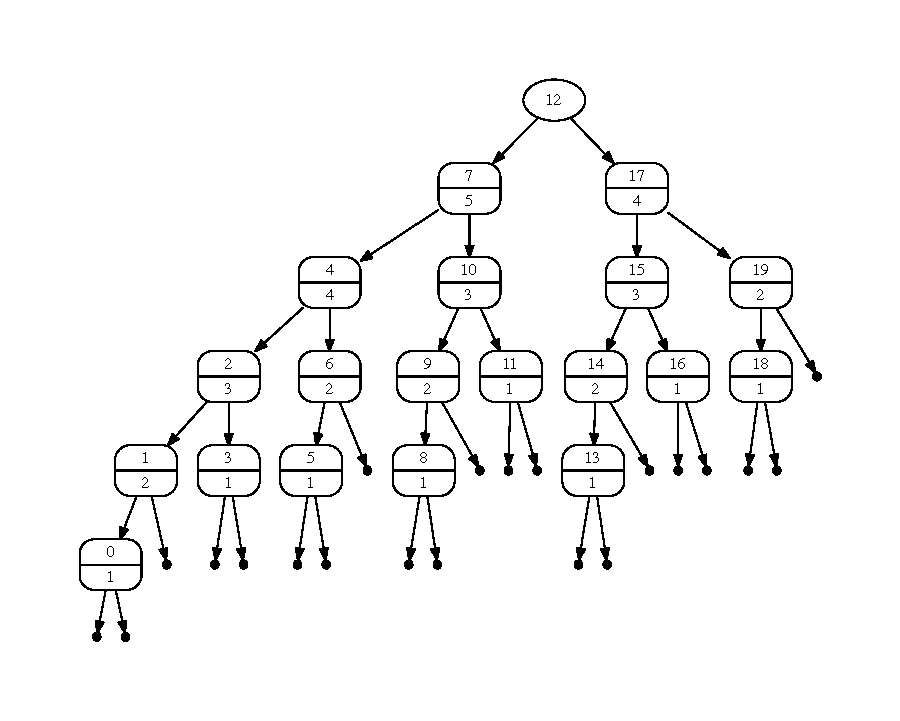
\epsfig{file=avl}} 
  \caption{Ein AVL-Baum mit dem ung\"unstigsten Verh\"altnis von H\"ohe zur Anzahl an Knoten}
  \label{fig:avl-worst-case}
\end{figure}
\pagebreak
\vspace*{\fill}

\pagebreak


\section{Tries}
In der Praxis kommt es h\"aufig vor, dass die Schl\"ussel des ADT \textsl{Map} Strings sind.
In dem einf\"uhrenden Beispiel des elektronischen Telefon-Buchs ist dies der Fall.  Es gibt eine
Form von Such-B\"aumen, die auf diese Situation besonders angepasst ist.  Diese Such-B\"aume
haben den Namen \emph{Tries}.  Dieses Wort ist von dem Englischen Wort
\emph{re\underline{trie}val} abgeleitet. Damit man \emph{Tries} und \emph{Trees}
unterscheiden kann, wird \emph{Trie} so ausgesprochen, dass es sich mit dem Englischen
Wort \emph{pie} reimt.  Diese Datenstruktur wurde 1959 von Ren\'e de la Briandais
\cite{briandais:59} vorgeschlagen.


Die Grundidee bei der Datenstruktur \emph{Trie} ist ein Baum, an dem jeder Knoten nicht
nur zwei Nachfolger hat, wie das bei bin\"aren B\"aumen der Fall ist, sondern statt dessen
potentiell f\"ur jeden Buchstaben des Alphabets einen Ast besitzt.  Um Tries definieren zu
k\"onnen, nehmen wir zun\"achst an, dass folgendes gegeben ist:
\begin{enumerate}
\item $\Sigma$ ist eine endliche Menge, deren Elemente wir als \emph{Buchstaben}
      bezeichnen. $\Sigma$ selbst hei{\ss}t das \emph{Alphabet}.
\item $\Sigma^*$ bezeichnet die Menge der \emph{W\"orter} (engl.~\emph{strings}), die wir aus den Buchstaben
      des Alphabets bilden k\"onnen.  Mathematisch k\"onnen wir W\"orter als Listen von 
      Buchstaben auffassen. Ist $w \in \Sigma^*$ so schreiben wir $w = cr$, falls
      $c$ der erste Buchstabe von $w$ ist und $r$ das Wort ist, das durch L\"oschen des
      ersten Buchstabens aus $w$ entsteht.  

      In \textsl{Java} k\"onnen wir sp\"ater $c$ und $r$ wie
      folgt aus dem String $w$ gewinnen: \\[0.2cm]
      \hspace*{1.3cm} $c = w.\textsl{charAt}(0)\mathtt{;}$ 
      \quad und \quad $r = w.\textsl{substring}(1)\mathtt{;}$
\item $\varepsilon$ bezeichnet das leere Wort.  In \textsl{Java} k\"onnen wir schreiben \\[0.2cm]
      \hspace*{1.3cm} $\mathtt{epsilon} = \symbol{34}\symbol{34}\mathtt{;}$ 
\item \textsl{Value} ist eine Menge von \emph{Werten}.  
\end{enumerate}
Die Menge $\mathbb{T}$ der Tries definieren wir nun induktiv mit Hilfe des 
Konstruktors \\[0.2cm]
\hspace*{1.3cm} 
$\textsl{node}: \textsl{Value} \times \textsl{List}(\Sigma) \times
\textsl{List}(\mathbb{T}) \rightarrow \mathbb{T}$. \\[0.2cm]
Die induktive Definition besteht nur aus einer einzigen Klausel. Falls
\begin{enumerate}
\item $v \in \textsl{Value} \cup \{\Omega\}$
\item $C = [c_1, \cdots, c_n] \in \textsl{List}(\Sigma)$ eine Liste von Buchstaben der
      L\"ange $n$ ist,
\item $T = [t_1, \cdots, t_n] \in \textsl{List}(\mathbb{T})$ eine Liste von Tries derselben L\"ange $n$ ist, 
\end{enumerate}
dann gilt \\[0.2cm]
\hspace*{1.3cm}  $\textsl{node}(v, C, T) \in \mathbb{T}$.  \\[0.2cm]
Als erstes fragen Sie sich
vermutlich, wo bei dieser induktiven Definition der Induktions-Anfang ist.
Der Induktions-Anfang ist der Fall $n=0$, denn dann sind die Listen $L$ und $T$ leer.

Als n\"achstes \"uberlegen wir uns, welche Funktion von dem Trie \\[0.2cm]
\hspace*{1.3cm}  $\textsl{node}(v, [c_1, \cdots, c_n], [t_1, \cdots, t_n]) \in \mathbb{T}$ \\[0.2cm]
dargestellt wird.  Wir beantworten diese Frage, indem wir rekursive Gleichungen f\"ur die
Methode \\[0.2cm]
\hspace*{1.3cm} $\textsl{find}: \mathbb{T} \times \Sigma^* \rightarrow \textsl{Value} \cup \{ \Omega\}$
\\[0.2cm]
angeben.  Wir werden den Ausdruck $\textsl{node}(v,L,T).\textsl{find}(s)$ durch Induktion \"uber den String $s$
definieren:
\begin{enumerate}
\item $\textsl{node}(v, C, T).\textsl{find}(\varepsilon) = v$.

      Der dem leeren String zugeordnete Wert wird also unmittelbar an der Wurzel
      des Tries abgespeichert.
\item $\textsl{node}(v, [c_1, \cdots, c_n], [t_1, \cdots, t_n]).\textsl{find}(cr) = 
        \left\{
        \begin{array}{ll}
        t_1.\textsl{find}(r) & \mbox{falls} \quad c = c_1 \mbox{;} \\
        \vdots &                                     \\
        t_i.\textsl{find}(r) & \mbox{falls} \quad c = c_i \mbox{;} \\
        \vdots &                                     \\
        t_n.\textsl{find}(r) & \mbox{falls} \quad c = c_n \mbox{;} \\[0.2cm]
        \Omega               & \mbox{falls} \quad c \notin \{c_1,\cdots,c_n\} \mbox{.}         
        \end{array}
       \right.$

      Der Trie $\textsl{node}(v, [c_1, \cdots, c_n], [t_1, \cdots, t_n])$ enth\"alt also genau
      dann einen Wert zu dem Schl\"ussel $cr$, wenn einerseits der Buchstabe $c$ in der Buchstaben-Liste
      an der Stelle $i$ auftritt und wenn andererseits der Trie $t_i$ einen Wert zu dem
      Schl\"ussel $r$ enth\"alt.
\end{enumerate}

\begin{figure}[!ht]
  \centering
  \framebox{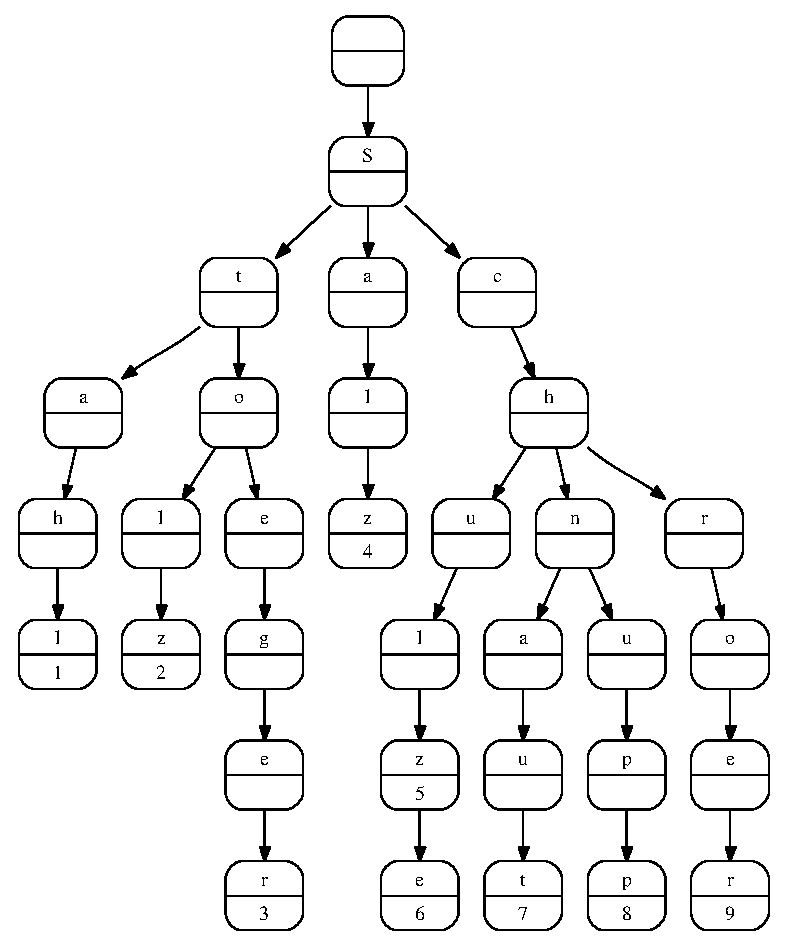
\epsfig{file=trie}} 
  \caption{Ein Beispiel Trie}
  \label{fig:trie}
\end{figure}

Zum besseren Verst\"andnis wollen wir Tries graphisch als B\"aume darstellen.
Nun ist es nicht sinnvoll, die Knoten dieser B\"aume mit langen Listen zu beschriften.
Wir behelfen uns mit einem Trick.  Um einen Knoten der Form \\[0.2cm]
\hspace*{1.3cm} 
$\textsl{node}(v, [c_1, \cdots, c_n], [t_1, \cdots, t_n])$ \\[0.2cm]
darzustellen, zeichnen wir einen Kreis,
den wir durch einen horizontalen Strich in der Mitte aufteilen.
Falls $v$ von $\Omega$ verschieden ist, schreiben wir den Wert $v$ in die untere H\"alfte
des Kreises.
(Bei den in Abbildung \ref{fig:trie} gezeigten Kreisen handelt es sich um
Mutantenkreise.)
Das, was wir \"uber dem Strich schreiben,
h\"angt von dem Vater des jeweiligen Knotens ab.  Wie genau es vom Vater abh\"angt, sehen wir gleich.
Der Knoten selber hat $n$ Kinder. Diese $n$ Kinder sind die 
Wurzeln der B\"aume, die die Tries $t_1$, $\cdots$, $t_n$ darstellen.
Au{\ss}erdem markieren wir die diese Knoten darstellenden Kreise in den oberen H\"alfte 
mit den Buchstaben $c_1$, $\cdots$, $c_n$.  


Zur Verdeutlichung geben wir ein Beispiel in 
Abbildung \ref{fig:trie} auf Seite \pageref{fig:trie}.
Die Funktion, die hier dargestellt wird, l\"asst sich wie folgt als bin\"are Relation
schreiben: \\[0.2cm]
\hspace*{1.3cm} $ \bigl\{ \langle \textrm{``Stahl''},   1  \rangle, \langle \textrm{``Stolz''},     2  \rangle, \langle \textrm{``Stoeger''},   3  \rangle, 
             \langle \textrm{``Salz''},      4  \rangle, \langle \textrm{``Schulz''},    5  \rangle$, \\[0.2cm]
\hspace*{1.5cm} $\langle \textrm{``Schulze''},   6  \rangle, \langle \textrm{``Schnaut''},   7  \rangle, 
  \langle \textrm{``Schnupp''},   8  \rangle, 
  \langle \textrm{``Schroer''},   9  \rangle\}$. \\[0.2cm]
Der Wurzel-Knoten ist hier leer, denn dieser Knoten hat keinen Vater-Knoten, von dem er
eine Markierung erben k\"onnte.  Diesem Knoten entspricht der Term \\[0.2cm]
\hspace*{1.3cm} $\textsl{node}(\Omega,[\textrm{`S'}], [t])$. \\[0.2cm]
Dabei bezeichnet $t$ den Trie, dessen Wurzel mit dem Buchstaben `S' markiert ist.
Diesen Trie k\"onnen wir seinerseits durch den Term \\[0.2cm]
\hspace*{1.3cm} 
$\textsl{node}(\Omega,[\textrm{`t'},\textrm{`a'},\textrm{`c'}], [t_1, t_2, t_3])$ \\[0.2cm]
darstellen.  Daher hat dieser Knoten drei S\"ohne, die mit den Buchstaben `t', `a' und `c'
markiert sind.

\subsection{Einf\"ugen in Tries}
Wir stellen nun bedingte Gleichungen auf, mit denen wir das Einf\"ugen eines Schl\"ussels mit
einem zugeh\"origen Wert beschreiben k\"onnen.  Bezeichnen wir die Methode f\"ur das Einf\"ugen
mit $\textsl{insert}()$, so hat diese Methode die Signatur
\\[0.2cm]
\hspace*{1.3cm}
$\textsl{insert}: \mathbb{T} \times \Sigma^* \times V \rightarrow \mathbb{T}$.
\\[0.2cm]
Wir definieren den Wert von \\[0.2cm]
\hspace*{1.3cm} $\textsl{node}(v, [c_1, \cdots, c_n], [t_1, \cdots, t_n]).\textsl{insert}(s,v)$\\[0.2cm]
f\"ur ein Wort $w\in \Sigma^*$ und einen Wert $v \in V$
durch Induktion nach der L\"ange des Wortes $w$.
\begin{enumerate}
\item $\textsl{node}(v_1,L,T).\textsl{insert}(\varepsilon, v_2) = \textsl{node}(v_2,L,T)$,

      Einf\"ugen eines Wertes mit dem leeren String als Schl\"ussel \"uberschreibt also einfach
      den an dem Wurzel-Knoten gespeicherten Wert. 
\item $\textsl{node}\bigl(v_1,[c_1,\cdots,c_i,\cdots,c_n], [t_1,\cdots,t_i,\cdots,t_n]\bigr).\textsl{insert}(c_ir,v_2) =$ \\[0.2cm]
      \hspace*{1.3cm}  
      $\textsl{node}\bigl(v_1,[c_1,\cdots,c_i,\cdots,c_n], [t_1,\cdots,t_i.\textsl{insert}(r,v_2),\cdots,t_n]\bigr)$.

      Wenn in dem Trie $\textsl{node}\bigl(v_1,[c_1,\cdots,c_i,\cdots,c_n], [t_1,\cdots,t_i,\cdots,t_n]\bigr)$ ein Wert
      $v_2$ zu dem Schl\"ussel $cr$ eingef\"ugt werden soll, und falls der Buchstabe $c$ in der Liste $[c_1,\cdots,c_n]$
      an der Stelle $i$ vorkommt, wenn also gilt $c= c_i$, dann muss der Wert $v_2$
      rekursiv in dem Trie $t_i$ unter dem Schl\"ussel 
      $r$ eingef\"ugt werden.

\item $c \not\in\{c_1,\cdots,c_n\} \;\rightarrow\;\textsl{node}\bigl(v_1,[c_1,\cdots,c_n], [t_1,\cdots,t_n]\bigr).\textsl{insert}(cr,v_2) =$ \\[0.2cm]
      \hspace*{1.3cm}  
      $\textsl{node}\bigl(v_1,[c_1,\cdots,c_n,c], [t_1,\cdots,t_n,\textsl{node}(\Omega,[],[]).\textsl{insert}(r,v_2)]\bigr)$.
      
      Wenn in dem Trie $\textsl{node}\bigl(v_1,[c_1,\cdots,c_n], [t_1,\cdots,t_n]\bigr)$
      ein Wert $v_2$ zu dem Schl\"ussel $cr$ eingef\"ugt werden soll, und falls der Buchstabe
      $c$ in der Liste $[c_1,\cdots,c_n]$ nicht vorkommt, dann wird zun\"achst ein Trie
      erzeugt, der die leere Abbildung repr\"asentiert.  Dieser Trie hat die Form \\[0.2cm]
      \hspace*{1.3cm} $\textsl{node}(\Omega, [], [])$. \\[0.2cm]
      Anschlie{\ss}end wird in diesem Trie der Wert $v_2$ rekursiv unter dem Schl\"ussel $r$
      eingef\"ugt. Zum Schluss h\"angen wir den Buchstaben $c$ an die Liste $[c_1,\cdots,c_n]$
      an und f\"ugen den Trie  \\[0.2cm] 
      \hspace*{1.3cm} $\textsl{node}(\Omega, [], []).\textsl{insert}(r,v_2)$ \\[0.2cm]
      am Ende der Liste $[t_1,\cdots,t_n]$ ein.
\end{enumerate}

\subsection{L\"oschen in Tries}
Als letztes stellen wir die bedingten Gleichungen auf, die das L\"oschen von
Schl\"usseln und den damit verkn\"upften Werten in einem Trie beschreiben.
Um diese Gleichungen einfacher schreiben zu k\"onnen, definieren wir zun\"achst eine
Hilfs-Funktion \\[0.2cm]
\hspace*{1.3cm} $\textsl{isEmpty}: \mathbb{T} \rightarrow \mathbb{B}$, \\[0.2cm]
so dass $t.\textsl{isEmpty}()$ genau dann $\mathtt{true}$ liefert, wenn der Trie
$t$ die leere Funktion darstellt.  Wir definieren also: 
\begin{enumerate}
\item $\textsl{node}(\Omega, [],[]).\textsl{isEmpty}() = \mathtt{true}$
\item $v \not= \Omega \rightarrow 
       \textsl{node}(v, [c_1,\cdots,c_n],[t_1,\cdots,t_n]).\textsl{isEmpty}() = \mathtt{false}$
\item $\textsl{node}(\Omega, L, T).\textsl{isEmpty}() = \textsl{isEmptyList}(T)$
\end{enumerate}
In der letzten Gleichung haben wir eine weitere Hilfs-Funktion benutzt, die wir noch
definieren m\"ussen.  Die Funktion
\\[0.2cm]
\hspace*{1.3cm}
$\textsl{isEmptyList}: \textsl{List}(\mathbb{T}) \rightarrow \mathbb{B}$
\\[0.2cm]
pr\"uft f\"ur eine gegebene Liste von Tries, ob alle in der Liste vorhandenen Tries leer sind.
Die Definition dieser Funktion erfolgt durch Induktion \"uber die L\"ange der Liste.
\begin{enumerate}
\item $\textsl{isEmptyList}\bigl([]\bigr) = \mathtt{true}$,
\item $\textsl{isEmptyList}\bigl([t] + R\bigr) = 
       \bigl(t.isEmpty() \wedge \textsl{isEmptyList}(R)\bigr)$,

      denn alle Tries in der Liste $[t]+R$ sind leer, wenn einerseits $t$ ein leerer
      Trie ist und wenn andererseits auch alle Tries in $R$ leer sind.
\end{enumerate}
Nun k\"onnen wir die Methode
\\[0.2cm]
\hspace*{1.3cm}
$\textsl{delete}: \mathbb{T} \times \Sigma^* \rightarrow \mathbb{T}$
\\[0.2cm]
spezifizieren:  Wir definieren den Wert von \\[0.2cm]
\hspace*{1.3cm} 
$t.\textsl{delete}(w)$
\\[0.2cm]
f\"ur einen Trie $t \in \mathbb{B}$ und ein Wort $w \in \Sigma^*$
durch Induktion nach der L\"ange des Wortes $w$.
\begin{enumerate}
\item $\textsl{node}(v,L,T).\textsl{delete}(\varepsilon) = \textsl{node}(\Omega,L,T)$,

      denn der Wert, der unter dem leeren String $\varepsilon$ in einem Trie
      gespeichert wird, befindet sich unmittelbar an der Wurzel des Tries und
      kann dort sofort gel\"oscht werden.
\item $\begin{array}[t]{ll}
       t_i.\textsl{delete}(r).\textsl{isEmpty}()   & \rightarrow \\
       \textsl{node}(v, [c_1,\cdots,c_i,\cdots,c_n],[t_1,\cdots,t_i,\cdots,t_n]).\textsl{delete}(c_ir) 
       & = \\
       \qquad 
       \textsl{node}(v, [c_1,\cdots,c_{i-1},c_{i+1},\cdots,c_n],[t_1,\cdots,t_{i-1},t_{i+1},\cdots,t_n]).
       \end{array}
       $

       Wenn der zu l\"oschende String mit dem Buchstaben $c_i$ anf\"angt, und wenn
       das L\"oschen des Schl\"ussels $r$ in dem $i$-ten Trie $t_i$ einen leeren
       Trie ergibt, dann streichen wir den $i$-ten Buchstaben und den dazu
       korrespondierenden $i$-ten Trie $t_i$.
\item $\begin{array}[t]{ll}
       \neg t_i.\textsl{delete}(r).\textsl{isEmpty}()   & \wedge \\
       \textsl{node}(v, [c_1,\cdots,c_i,\cdots,c_n],[t_1,\cdots,t_i,\cdots,t_n]).\textsl{delete}(c_ir) 
       & = \\
       \qquad \textsl{node}(v, [c_1,\cdots,c_i,\cdots,c_n],[t_1,\cdots,t_i.\textsl{delete}(r),\cdots,t_n]).
       \end{array}
       $

       Wenn der zu l\"oschende String mit dem Buchstaben $c_i$ anf\"angt, und wenn
       der Baum $t_i$, der durch das  L\"oschen des Schl\"ussels $r$ in dem $i$-ten
       Trie $t_i$ entsteht nicht leer ist, dann l\"oschen wir rekursiv in dem Baum $t_i$ den Schl\"ussel
       $r$.
\item $c \notin C \rightarrow \textsl{node}(v, C, T).\textsl{delete}(cr) = \textsl{node}(v, C, T)$.

       Wenn der zu l\"oschende String mit dem Buchstaben $c$ anf\"angt und wenn der
       Buchstabe $c$ gar kein Element der Buchstaben-Liste $C$ des Tries
       ist, dann ver\"andert das L\"oschen den Trie nicht.
\end{enumerate}

\subsection{Implementierung in \textsl{Java}}
Wir zeigen nun, wie sich die Tries in \textsl{Java} implementieren lassen.
Die Abbildungen \ref{fig:TrieNode-I} und \ref{fig:TrieNode-II} auf den Seiten
\pageref{fig:TrieNode-I} und 
\pageref{fig:TrieNode-II} zeigen die Implementierung, die wir jetzt diskutieren.

\begin{figure}[!ht]
  \centering
\begin{Verbatim}[ frame         = lines, 
                  framesep      = 0.3cm, 
                  labelposition = bottomline,
                  numbers       = left,
                  numbersep     = -0.2cm,
                  xleftmargin   = 0.2cm,
                  xrightmargin  = 0.2cm
                ]
    import java.util.*;
    
    public class TrieNode<Value> implements MyMap<String, Value>
    {
        Value                      mValue;
        ArrayList<Character>       mCharList;
        ArrayList<TrieNode<Value>> mNodeList;
    
        TrieNode() {
            mValue    = null;
            mCharList = new ArrayList<Character>(0);
            mNodeList = new ArrayList<TrieNode<Value>>(0);
        }    
        public Value find(String key) {
            if (key.length() == 0) {
                return mValue;
            } else {
                Character firstChar = key.charAt(0);
                String    rest      = key.substring(1);
                for (int i = 0; i < mCharList.size(); ++i) {
                    if (firstChar.equals(mCharList.get(i))) {
                        return mNodeList.get(i).find(rest);
                    }
                }
                return null;
            }
        }
        public void insert(String key, Value value) {
            if (key.length() == 0) {
                mValue = value;
            } else {
                Character firstChar = key.charAt(0);
                String    rest      = key.substring(1);
                for (int i = 0; i < mCharList.size(); ++i) {
                    if (firstChar.equals(mCharList.get(i))) {
                        mNodeList.get(i).insert(rest, value);
                        return;
                    }
                }
                mCharList.add(firstChar);
                TrieNode<Value> node = new TrieNode<Value>();
                node.insert(rest, value);
                mNodeList.add(node);
            }
        }
\end{Verbatim}
\vspace*{-0.3cm}
  \caption{Die Klasse \textsl{TrieNode-I}, Teil \texttt{I}.}
  \label{fig:TrieNode-I}
\end{figure}

\begin{enumerate}
\item Den Trie $\textsl{node}(v, [c_1,\cdots,c_n], [t_1,\cdots,t_n])$ stellen wir durch ein Objekt der Klasse
      \textsl{TrieNode} dar.  Diese Klasse hat drei Member-Variablen:
      \begin{enumerate}
      \item \texttt{mValue} entspricht dem Wert $v$, der an der Wurzel des Tries
             gespeichert ist.
      \item \texttt{mCharList} entspricht der Buchstaben-Liste $[c_1,\cdots,c_n]$.
      \item \texttt{mNodeList} entspricht der Trie-Liste $[t_1,\cdots,t_n]$.
      \end{enumerate}
\item Der Konstruktor in Zeile 9 erzeugt den Trie $\textsl{node}(\Omega, [], [])$, der die
      leere Funktion repr\"asentiert.
\item Die Implementierung der Methode \textsl{find} orientiert sich genau an den Gleichungen, 
      mit denen wir diese Methode spezifiziert haben.
      \begin{enumerate}
      \item Falls der Schl\"ussel, nach dem wir suchen, der leere String ist,
            geben wir den Wert \texttt{mValue} zur\"uck.
      \item Sonst hat der Schl\"ussel die Form $\textsl{key} = cr$. Wir setzen
            $\textsl{firstChar} = c$ und $\textsl{rest} = r$.  Wir gehen nun die
            Buchstaben-Liste \texttt{mCharList} durch und schauen, ob wir 
            dabei den Buchstaben $c$ finden.  Wenn  wir den Buchstaben $c$ an der $i$-ten
            Stelle finden, dann suchen wir anschlie{\ss}end  in dem $i$-ten Trie in der Liste 
            \texttt{mNodeList} nach dem Schl\"ussel $r$.

            Falls der Buchstabe $c$ nicht gefunden wird, geben wir \texttt{null} zur\"uck um
            den speziellen Wert $\Omega$ zu repr\"asentieren.
      \end{enumerate}
\item Die Implementierung der Methode \textsl{insert} ist analog zu der Implementierung
      der Methode \textsl{find}.
      \begin{enumerate}
      \item Falls der Schl\"ussel, unter dem wir den Wert \textsl{value} einf\"ugen wollen, der
            leere String ist, k\"onnen  wir die Member-Variable \texttt{mValue} \"uberschreiben.
      \item Sonst hat der Schl\"ussel die Form $\textsl{key} = cr$. Wir setzen wieder
            $\textsl{firstChar} = c$ und $\textsl{rest} = r$.  Wir gehen nun die
            Buchstaben-Liste \texttt{mCharList} durch und suchen den Buchstaben $c$.  
            Wenn wir $c$ an der $i$-ten
            Stelle finden, dann f\"ugen wir anschlie{\ss}end  in dem $i$-ten Trie in der Liste 
            \texttt{mNodeList} den Wert \texttt{value} unter dem Schl\"ussel $r$ ein.

            Falls der Buchstabe $c$ nicht in der Liste \texttt{mCharList} auftritt,
            dann f\"ugen wir $c$ am Ende der Buchstaben-Liste ein.  Gleichzeitig erzeugen
            wir einen zun\"achst leeren Trie, in dem wir dann den Wert \texttt{value} unter dem
            Schl\"ussel $r$ einf\"ugen.  Diesen Trie f\"ugen wir an das Ende der Liste
            \texttt{mNodeList} ein.            
      \end{enumerate}
\item Als letztes diskutieren wir die Implementierung der Methode \textsl{delete}.
      \begin{enumerate}
      \item Falls der Schl\"ussel, den wir l\"oschen wollen, der
            leere String ist, so setzen wir einfach die Member-Variable \texttt{mValue}
            auf \texttt{null}.
      \item Sonst hat der Schl\"ussel die Form $\textsl{key} = cr$. Wir setzen wieder
            $\textsl{firstChar} = c$ und $\textsl{rest} = r$.  Wir gehen nun die
            Buchstaben-Liste \texttt{mCharList} durch und suchen den Buchstaben $c$
            finden.  Wenn wir $c$ an der $i$-ten 
            Stelle finden, dann l\"oschen wir in dem $i$-ten Trie in der Liste 
            \texttt{mNodeList} den Schl\"ussel $r$.  Falls dieser Trie jetzt leer ist,
            so l\"oschen wir einerseits diesen Trie aus \texttt{mNodeList} und andererseits
            l\"oschen wir den Buchstaben $c_i$ aus der Liste \texttt{mCharList}.

            Falls der Buchstabe $c$ nicht in der Liste \texttt{mCharList} auftritt,
            so ist nichts weiter zu tun, denn in diesem Fall sind in dem Trie keinerlei
            Informationen zu dem Schl\"ussel \textsl{key} gespeichert.
      \end{enumerate}
\end{enumerate}

\begin{figure}[!ht]
  \centering
\begin{Verbatim}[ frame         = lines, 
                  framesep      = 0.3cm, 
                  firstnumber   = last,
                  labelposition = bottomline,
                  numbers       = left,
                  numbersep     = -0.2cm,
                  xleftmargin   = 0.2cm,
                  xrightmargin  = 0.2cm
                ]
        public void delete(String key) {
            if (key.length() == 0) {
                mValue = null;
                return;
            } 
            Character firstChar = key.charAt(0);
            String    rest      = key.substring(1);
            for (int i = 0; i < mCharList.size(); ++i) {
                if (firstChar.equals(mCharList.get(i))) {
                    TrieNode<Value> node = mNodeList.get(i);
                    node.delete(rest);
                    if (node.isEmpty()) {
                        mCharList.remove(i);
                        mNodeList.remove(i);
                    } 
                    return;
                }
            }
        }
        public Boolean isEmpty() {
            return mValue == null && mNodeList.size() == 0;
        }
    }
\end{Verbatim}
\vspace*{-0.3cm}
  \caption{Die Klasse \textsl{TrieNode}, Teil \texttt{II}.}
  \label{fig:TrieNode-II}
\end{figure}

\noindent
\textbf{Bemerkung}:  Falls das Alphabet $\Sigma$ viele Buchstaben enth\"alt, 
k\"onnen die Listen $[c_1, \cdots, c_n]$ und $[t_1,\cdots,t_n]$, die in einem Trie  der Form
\\[0.2cm]
\hspace*{1.3cm}
$\textsl{node}(v, [c_1, \cdots, c_n], [t_1,\cdots,t_n])$
\\[0.2cm]
abgespeichert sind, lang werden.  Dann ist es eventuell effizienter, die Buchstaben-Liste
$[c_1, \cdots, c_n]$ zu sortieren.  Dann k\"onnte die Methode $\textsl{find}()$
effizienter implementiert werden.  Allerdings wird das Einf\"ugen und L\"oschen in diesem Fall komplizierter.
\vspace*{0.3cm}


\noindent
\textbf{Bin\"are Tries}:  Wir nehmen im Folgenden an, dass unser Alphabet nur aus den beiden
Ziffern $0$ und $1$ besteht, es gilt also $\Sigma = \{0,1\}$.  Dann k\"onnen wir nat\"urliche
Zahlen als Worte aus $\Sigma^*$ auffassen.  Wir wollen die Menge der \emph{bin\"aren Tries}
mit $\BT$ bezeichnen und wie folgt induktiv definieren:
\begin{enumerate}
\item $\textsl{nil} \in \BT$.
\item $\textsl{bin}(v,l,r) \in \BT$ falls
      \begin{enumerate}
      \item $v \in \textsl{Value} \cup \{\Omega\}$.
      \item $l,r \in \BT$.
      \end{enumerate}
\end{enumerate}
Die Semantik legen wir fest, indem wir eine Methode 
\\[0.2cm]
\hspace*{1.3cm}
$\textsl{find}: \BT \times \mathbb{N} \rightarrow \textsl{Value} \cup \{ \Omega \}$
\\[0.2cm]
definieren.  F\"ur einen bin\"aren Trie $b$ und eine nat\"urliche Zahl $n$ gibt
$b.\textsl{find}(n)$ den Wert zur\"uck, der unter dem Schl\"ussel $n$ in dem bin\"aren Trie $b$ gespeichert ist.
Falls in dem bin\"aren Trie $b$ unter dem Schl\"ussel $n$ kein Wert gespeichert ist, wird
$\Omega$ zur\"uck gegeben.
Formal definieren wir den Wert von $b.\textsl{find}(n)$ durch Induktion nach dem Aufbau
von $b$.  Im Induktions-Schritt ist eine Neben-Induktion nach $n$ erforderlich.
\begin{enumerate}
\item $\textsl{nil}.\textsl{find}(n) = \Omega$,

      denn in dem leeren bin\"aren Trie finden wir keine Werte.
\item $\textsl{bin}(v,l,r).\textsl{find}(0) = v$,

      denn der Schl\"ussel $0$ entspricht dem leeren String $\varepsilon$.
\item $n \not= 0 \rightarrow \textsl{bin}(v,l,r).\textsl{find}(2\!\cdot \!n) = l.\textsl{find}(n)$,

      denn wenn wir Zahlen im Bin\"arsystem darstellen, so hat bei geraden Zahlen das letzte
      Bit den Wert 0 und die 0 soll dem linken Teilbaum entsprechen.
\item $\textsl{bin}(v,l,r).\textsl{find}(2\!\cdot \!n\!+\!1) = r.\textsl{find}(n)$,

      denn wenn wir Zahlen im Bin\"arsystem darstellen, so hat bei ungeraden Zahlen das letzte
      Bit den Wert 1 und die 1 soll dem rechten Teilbaum entsprechen.
\end{enumerate}
\textbf{Aufgabe}: 
\begin{enumerate}
\item Stellen Sie Gleichungen auf, die das Einf\"ugen und das L\"oschen in einem
      bin\"aren Trie beschreiben.  Achten Sie beim L\"oschen darauf,
      dass bin\"are Tries der Form $\textsl{bin}(\Omega, \textsl{nil}, \textsl{nil})$
      zu $\textsl{nil}$ vereinfacht werden.

      \textbf{Hinweis}:  Um die Gleichungen zur Spezifikation der Funktion
      $\textsl{delete}()$ nicht zu komplex werden zu lassen ist es sinnvoll, eine
      Hilfsfunktion zur Vereinfachung von bin\"aren Tries zu definieren.
\item Implementieren Sie bin\"are Tries in \textsl{Java}.
\end{enumerate}
\textbf{Bemerkung}: Bin\"are Tries werden auch als \emph{digitale Suchb\"aume} bezeichnet.
\pagebreak


\section{Hash-Tabellen}
Eine Abbildung \\[0.2cm]
\hspace*{1.3cm} $f: \textsl{Key} \rightarrow \textsl{Value}$ \\[0.2cm]
kann dann sehr einfach implementiert werden, wenn \\[0.2cm]
\hspace*{1.3cm} $\textsl{Key} = \{ 0, 1, 2, \cdots, n \}$, \\[0.2cm]
denn dann reicht es aus, ein Feld der Gr\"o{\ss}e $n+1$ zu verwenden.
Abbildung \ref{fig:ArrayMap} zeigt, dass sich der ADT \textsl{Map} 
in diesem Fall trivial implementieren l\"asst.

\begin{figure}[!ht]
  \centering
\begin{Verbatim}[ frame         = lines, 
                  framesep      = 0.3cm, 
                  labelposition = bottomline,
                  numbers       = left,
                  numbersep     = -0.2cm,
                  xleftmargin   = 0.8cm,
                  xrightmargin  = 0.8cm
                ]
    public class ArrayMap<Value> implements MyMap<Integer, Value>
    {
        Value[] mArray;
        
        public ArrayMap(int n) {
            mArray = (Value[]) new Object[n+1];
        }
        public Value find(Integer key) {
            return mArray[key];
        }
        public void insert(Integer key, Value value) {
            mArray[key] = value;
        }
        public void delete(Integer key) {
            mArray[key] = null;
        }
    }
\end{Verbatim}
\vspace*{-0.3cm}
  \caption{Die Klasse \textsl{ArrayMap}.}
  \label{fig:ArrayMap}
\end{figure}


Falls nun der Definitions-Bereich $D$ der darzustellenden Abbildung nicht die Form einer
Menge der Gestalt $\{1, \cdots, n\}$ hat, 
k\"onnten wir versuchen, $D$ zun\"achst auf eine Menge der Form $\{1,\cdots,n\}$ abzubilden.
Wir erl\"autern diese Idee  an einem einfachen Beispiel.
Wir betrachten eine naive Methode um ein Telefon-Buch abzuspeichern:
\begin{enumerate}
\item Wir machen zun\"achst die Annahme, dass alle Namen aus genau  
      8 Buchstaben bestehen.  Dazu werden
      k\"urzere Namen mit Blanks aufgef\"ullt und Namen die l\"anger als 8 Buchstaben sind,
      werden nach dem  8-ten Buchstaben abgeschnitten.
\item Als n\"achstes \"ubersetzen wir Namen in einen Index.  
      Dazu fassen wir die einzelnen Buchstaben als Ziffern auf, die die Werte von 0 bis 26
      annehmen k\"onnen.  Dem Blank ordnen wir dabei den Wert 0 zu.   Nehmen wir an, dass
      die Funktion $\textsl{ord}$ jedem Buchstaben aus der Menge 
      $\Sigma = \{ \texttt{' '}, \texttt{'a'}, \texttt{'b'}, \texttt{'c'}, \cdots, \texttt{'x'}, \texttt{'y'}, \texttt{'z'} \}$ 
      einen Wert aus der Menge
      $\{0,\cdots,26\}$ zuordnet \\[0.2cm]
      \hspace*{1.3cm} 
      $\textsl{ord}: \{ \texttt{' '}, \texttt{'a'}, \texttt{'b'}, \texttt{'c'}, \cdots, \texttt{'x'}, \texttt{'y'}, \texttt{'z'} \} \rightarrow \{0,\cdots, 26\}$,
      \\[0.2cm]
      so l\"asst sich der Wert eines Strings $w = c_0c_1\cdots c_7$ durch eine Funktion \\[0.2cm]
      \hspace*{1.3cm} 
      $\textsl{code}: \Sigma^* \rightarrow \mathbb{N}$ \\[0.2cm]
      berechnen, die wie folgt definiert ist: \\[0.2cm]
      \hspace*{1.3cm} 
      $\textsl{code}(c_0c_1\cdots c_7) = \sum\limits_{i=0}^7 \textsl{ord}(c_i) \cdot 27^i$.
      \\[0.2cm]
      Die Menge \textsl{code} bildet die Menge aller W\"orter mit 8 Buchstaben bijektiv
      auf die Menge der Zahlen $\{0,\cdots,(27^8 - 1)/26\}$ ab.
\end{enumerate}
Leider hat diese naive Implementierung mehrere Probleme: 
\begin{enumerate}
\item Das Feld, das wir anlegen m\"ussen, hat eine Gr\"o{\ss}e von \\[0.2cm]
      \hspace*{1.3cm} $27^8 = 282\,429\,536\,481$ \\[0.2cm]
      Eintr\"agen.  Selbst wenn jeder Eintrag nur die Gr\"o{\ss}e zweier Maschinen-Worte hat und
      ein Maschinen-Wort aus 4 Byte besteht, so br\"auchten wir 
      etwas mehr als ein Terabyte um eine
      solche Tabelle anzulegen.
\item Falls zwei Namen sich erst nach dem 8-ten Buchstaben unterscheiden, k\"onnen 
      wir zwischen diesen Namen nicht mehr unterscheiden. 
\end{enumerate}
Wir k\"onnen diese Probleme wir folgt l\"osen:
\begin{enumerate}
\item Wir \"andern die Funktion \texttt{code} so ab, dass das Ergebnis
      immer kleiner-gleich einer vorgegebene Zahl \texttt{size} ist.  Die Zahl
      \texttt{size} gibt dabei die Gr\"o{\ss}e eines Feldes an und ist so klein,
      dass wir ein solches Feld bequem anlegen k\"onnen.

      Eine einfache M\"oglichkeit, die Funktion \textsl{code} entsprechend abzu\"andern,
      besteht in folgender Implementierung: \\[0.2cm]
      \hspace*{1.3cm} 
      $\textsl{code}(c_0c_1\cdots c_n) = \left(\sum\limits_{i=0}^n \textsl{ord}(c_i) \cdot 27^i\right) \;\%\; \textsl{size}$.
      \\[0.2cm]
      Um eine \"Uberlauf zu vermeiden, k\"onnen wir f\"ur $k=n,n-1,\cdots,1,0$ die Teilsummen $s_k$
      wie folgt induktiv definieren:
      \begin{enumerate}
      \item $s_n = \textsl{ord}(c_n)$
      \item $s_{k} = \left(\textsl{ord}(c_{k}) + s_{k+1} \cdot 27 \right) \;\%\; \textsl{size}$
      \end{enumerate}
      Dann gilt
      \hspace*{1.3cm} 
      $s_0 = \left(\sum\limits_{i=0}^n \textsl{ord}(c_i) \cdot 27^i\right) \;\%\; \textsl{size}$.
      
\item In dem Feld der Gr\"o{\ss}e \textsl{size} speichern wir nun nicht mehr die Werte, sondern statt dessen
      Listen von Paaren aus Schl\"usseln und Werten.  Dies ist notwendig, denn wir k\"onnen
      nicht verhindern, dass die Funktion \texttt{code}() f\"ur zwei verschiedene
      Schl\"ussel den selben Index liefert.
\end{enumerate}
Abbildung \ref{fig:hash-example} auf Seite \pageref{fig:hash-example} zeigt, wie ein Feld,
in dem Listen von Paaren abgebildet sind, aussehen kann.  Ein solches Feld bezeichnen wir
als Hash-Tabelle.  Wir diskutieren nun die Implementierung dieser Idee in \textsl{Java}.


\begin{figure}[!ht]
  \centering
  \framebox{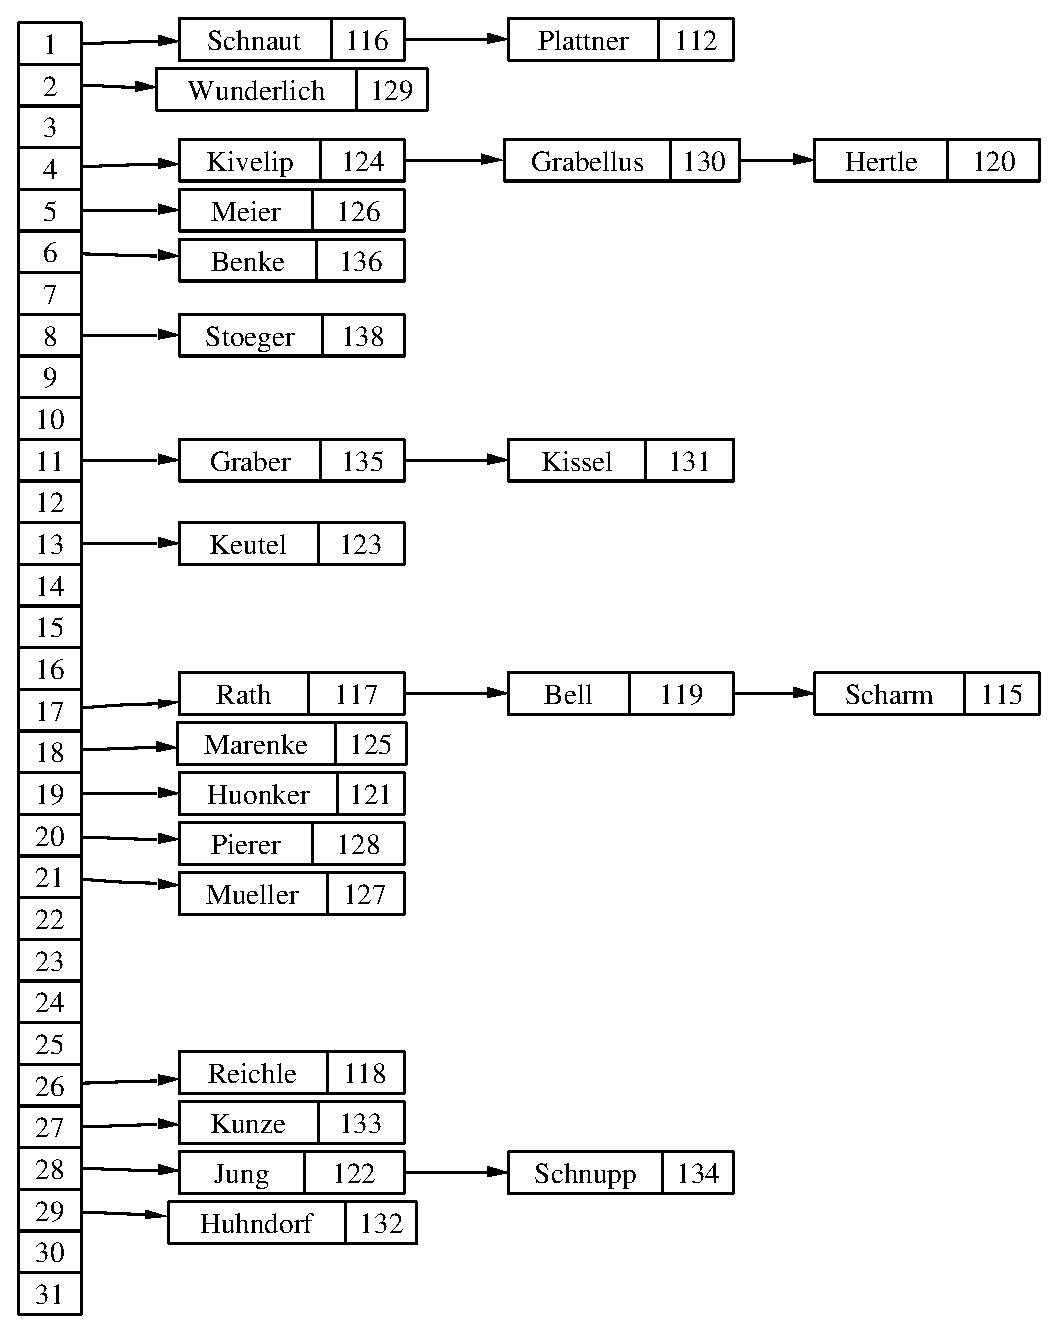
\epsfig{file=hash-table,scale=0.7}} 
  \caption{Eine Hash-Tabelle}
  \label{fig:hash-example}
\end{figure}


\begin{figure}[!ht]
  \centering
\begin{Verbatim}[ frame         = lines, 
                  framesep      = 0.3cm, 
                  labelposition = bottomline,
                  numbers       = left,
                  numbersep     = -0.2cm,
                  xleftmargin   = 0.0cm,
                  xrightmargin  = 0.0cm
                ]
    public class MyHashMap<Key, Value> implements MyMap<Key, Value>
    {
        static final double sAlpha = 2;
        static final int[] sPrimes = { 3, 7, 13, 31, 61, 127, 251, 
             509, 1021, 2039, 4093, 8191, 16381, 32749, 65521, 131071, 
             262139, 524287, 1048573, 2097143, 4194301, 8388593, 16777213, 
             33554393, 67108859, 134217689, 268435399, 536870909, 1073741789, 
             2147483647 
        };
        Object[] mArray;
        int      mPrimeIndex;
        int      mNumberEntries;
    
        public MyHashMap(int primeIndex) {
            mPrimeIndex = primeIndex;
            int size    = sPrimes[mPrimeIndex];
            mArray      = new Object[size];
        }
        public Value find(Key key) {
            int index = Math.abs(key.hashCode() % mArray.length);
            LinkedList<Pair<Key, Value>> list  = 
                (LinkedList<Pair<Key, Value>>) mArray[index];
            if (list == null) {
                return null;
            }
            for (int i = 0; i < list.size(); ++i) {
                Pair<Key, Value> pair = list.get(i);
                if (key.equals(pair.getFirst())) {
                    return pair.getSecond();
                }
            }
            return null;
        }
\end{Verbatim}
\vspace*{-0.3cm}
  \caption{Die Klasse \textsl{MyHashMap}, Teil \texttt{I}.}
  \label{fig:MyHashMap-I}
\end{figure}

\begin{figure}[!ht]
  \centering
\begin{Verbatim}[ frame         = lines, 
                  framesep      = 0.3cm, 
                  firstnumber   = last,
                  labelposition = bottomline,
                  numbers       = left,
                  numbersep     = -0.2cm,
                  xleftmargin   = 0.0cm,
                  xrightmargin  = 0.0cm
                ]
        public void insert(Key key, Value value) {
           if (mNumberEntries / (double) mArray.length > sAlpha) {
                rehash();
            }
            int index = Math.abs(key.hashCode() % mArray.length);
            LinkedList<Pair<Key, Value>> list  = 
                (LinkedList<Pair<Key, Value>>) mArray[index];
            if (list == null) {
                list          = new LinkedList<Pair<Key, Value>>();
                mArray[index] = list;
            }
            for (int i = 0; i < list.size(); ++i) {
                Pair<Key, Value> pair = list.get(i);
                if (key.equals(pair.getFirst())) {
                    pair.setSecond(value);
                    return;
                }
            }
            list.add(new Pair<Key, Value>(key, value));
            ++mNumberEntries;
        }
        private void rehash() {
            ++mPrimeIndex;
            MyHashMap<Key, Value> bigMap = new MyHashMap<Key, Value>(mPrimeIndex);
            for (Object list: mArray) {
                if (list == null) {
                    continue;
                }
                for (Object object: (LinkedList<Pair<Key, Value>>) list) {
                    Pair<Key, Value> pair = (Pair<Key, Value>) object;
                    bigMap.insert(pair.getFirst(), pair.getSecond());
                }
            }
            mArray = bigMap.mArray;
        }
\end{Verbatim}
\vspace*{-0.3cm}
  \caption{Die Klasse \textsl{MyHashMap}, Teil \texttt{II}.}
  \label{fig:MyHashMap-II}
\end{figure}


\begin{figure}[!ht] 
  \centering
\begin{Verbatim}[ frame         = lines, 
                  framesep      = 0.3cm, 
                  firstnumber   = last,
                  labelposition = bottomline,
                  numbers       = left,
                  numbersep     = -0.2cm,
                  xleftmargin   = 0.0cm,
                  xrightmargin  = 0.0cm
                ]
        public void delete(Key key) {
            int index = Math.abs(key.hashCode() % mArray.length);
            LinkedList<Pair<Key, Value>> list  = 
                (LinkedList<Pair<Key, Value>>) mArray[index];
            if (list == null) {
                return;
            }
            for (int i = 0; i < list.size(); ++i) {
                Pair<Key, Value> pair = list.get(i);
                if (key.equals(pair.getFirst())) {
                    list.remove(i);
                    --mNumberEntries;
                    return;
                }
            }
        }
    }
\end{Verbatim}
\vspace*{-0.3cm}
  \caption{Die Klasse \textsl{MyHashMap}, Teil \texttt{III}.}
  \label{fig:MyHashMap-III}
\end{figure}

\begin{enumerate}
\item Als erstes \"uberlegen wir uns, welche Daten-Strukturen wir brauchen,
      um eine Hash-Tabelle zu repr\"asentieren.
      \begin{enumerate}
      \item Wir ben\"otigen ein Feld, indem wir die einzelnen Listen ablegen.
            Dieses Feld wird in Zeile 10 als die Member-Variable \texttt{mArray}
            abgespeichert.

            Es mag Sie verwundern, dass dieses Feld den Typ \texttt{Object[]} hat.
            Eigentlich sollte dieses Feld in der Form \\[0.2cm]
            \hspace*{1.3cm} \texttt{List<Pair<Key, Value>>[] mArray;} \\[0.2cm]
            deklariert werden.  Die Erzeugung generischer Felder ist in \textsl{Java} 
            aber sehr trickreich.  Um nicht zu sehr vom eigentlichen Thema abzukommen
            haben wir daher eine Implementierung gew\"ahlt, die nicht Typ-sicher ist.
      \item Wenn die einzelnen Listen zu gro{\ss} werden, wird die Suche ineffizient.
            Daher ist es notwendig, die Gr\"o{\ss}e dieser Listen zu kontrollieren,
            wenn die Listen zu gro{\ss} werden, muss das Feld vergr\"o{\ss}ert werden.
            Um diesen Prozess zu steuern, m\"ussen wir zun\"achst nachhalten, 
            wieviele Elemente schon in der Hash-Tabelle abgespeichert sind.
            Dies geschieht in der Member-Variable \texttt{mNumberEntries}, die in Zeile 12
            definiert wird.

            Theoretische Untersuchungen, die \"uber den Rahmen der Vorlesung hinausgehen, zeigen, dass
            die Gr\"o{\ss}e der Tabelle eine Primzahl sein sollte.  Daher verf\"ugt der
            Konstruktor \"uber eine Liste von Primzahlen, 
            die in der statistischen Member-Variablen \texttt{sPrimes}, die in Zeile 4
            definiert ist, abgelegt sind.  
            Die $i+1$-te Primzahlen in dieser Liste ist in etwa doppelt so gro{\ss} wie die $i$-te
            Primzahl. Die Member-Variable \texttt{mPrimeIndex}, die
            in Zeile 11 definiert wird, kodiert nun die Gr\"o{\ss}e des
            Feldes \texttt{mArray}.  Es gilt immer \\[0.2cm]
            \hspace*{1.3cm} \texttt{mArray.length == sPrimes[mPrimeIndex]}. \\[0.2cm]
            Die durchschnittliche L\"ange der einzelnen Listen ergibt sich als
            der Quotient aus der Zahl \texttt{mNumberEntries} und der L\"ange des Feldes
            \texttt{mArray}.  Wird nun dieser Wert gr\"o{\ss}er als der
            \emph{Auslastungs-Faktor} (engl.~\emph{load factor})             
            \texttt{sAlpha}, der in Zeile 3 definiert ist, dann verdoppeln wir die Gr\"o{\ss}e
            des Feldes.
      \end{enumerate}
\item Der Konstruktor in Zeile 14 initialsiert \texttt{mPrimeIndex} mit dem gegebenen Argument.
      Wird der Konstruktor zum Beispiel mit dem Argument 0 aufgerufen, dann wird ein Feld
      der L\"ange 3 angelegt, denn es gilt $\texttt{sPrimes[0]} = 3$.
\item Bei der Implementierung der Methode \texttt{find} wandeln wir den gegebenen Schl\"ussel 
      \texttt{key} zun\"achst mit der Methode \texttt{hashCode}() in eine Zahl um.  
      Die Methode \texttt{hashCode}() ist in \textsl{Java} f\"ur jedes Objekt definiert
      und erzeugt eine mehr oder weniger zuf\"allige Zahl, die aber in eindeutiger Weise
      von dem Objekt abh\"angt.  Diese Zahl kann auch negativ sein.
      Wir modifizieren diese Zahl in Zeile 20 durch Bilden von Modulo und Absolutbetrag
      so, dass das Ergebnis in der Menge 
      $\{\,0,\; \cdots,\; \mathtt{mArray.length} - 1\,\}$ liegt.
      Anschlie{\ss}end holen wir die Liste, in der Werte zu dem gegebenen Schl\"ussel
      abgespeichert sein m\"ussen.  Falls in dem Feld an der Stelle, die durch den berechneten 
      Index angegeben wird, noch gar keine Liste gespeichert ist,
      hat die Hash-Tabelle zu dem gegebenen Schl\"ussel noch keinen Eintrag und wir geben in
      Zeile 24 \texttt{null} zur\"uck.

      Andernfalls laufen wir mit einer Schleife durch die Liste durch und vergleichen 
      die einzelnen Schl\"ussel mit dem gegebenen Schl\"ussel \texttt{key}.
      Falls wir den Schl\"ussel finden, geben wir in Zeile 29 den mit diesem Schl\"ussel
      assoziierten Wert zur\"uck.

      Falls wir die Schleife bis zum Ende durchlaufen und den Schl\"ussel nicht gefunden
      haben, dann hat die Hash-Tabelle zu dem gegebenen Schl\"ussel \texttt{key} keinen
      Eintrag und wir geben in Zeile 32 wieder \texttt{null} zur\"uck.

\item Bei der Implementierung der Methode \textsl{insert} berechnen wir zun\"achst den
      aktuellen Auslastungs-Faktor, also die durchschnittliche L\"ange der Listen.  Falls diese L\"ange
      gr\"o{\ss}er als der vorgegebene maximale Auslastungs-Faktor \texttt{sAlpha} ist,
      f\"uhren wir ein sogenanntes \emph{Rehashing} durch, das wir weiter unten im Detail
      diskutieren.

      Anschlie{\ss}end ist die Implementierung analog zur Implementierung der Methode
      \textsl{find}().  Wir berechnen also zun\"achst die Liste, in der Schl\"ussel
      \texttt{key} und der Wert \texttt{value} einzuf\"ugen sind.  Falls unter dem Index
      noch keine Liste existiert, erzeugen wir in den Zeilen 42 und 43 eine neue leere
      Liste und tragen diese Liste in das Feld ein.  

      Anschlie{\ss}end durchlaufen wir die Liste und suchen den Schl\"ussel \texttt{key}.
      Wenn wir den Schl\"ussel finden, dann wird einfach der zugeh\"orige Wert \"uberschrieben.
      Wenn wir den Schl\"ussel \texttt{key} in der Liste nicht finden, dann f\"ugen wir den
      Schl\"ussel zusammen mit dem zugeordneten Wert \texttt{value} in Zeile 52 an das Ende der Liste an.
      Gleichzeitig m\"ussen wir in diesem Fall die Zahl der Eintr\"age \texttt{mNumberEntries}
      inkrementieren.
\item Als n\"achstes besprechen wir das \emph{Rehashing}, das in Zeile 55 -- 69
      implementiert ist.  Wir inkrementieren zun\"achst \texttt{mPrimeIndex} und
      bilden dann eine neue Hash-Tabelle, die in etwa doppelt so gro{\ss} ist, wie die alte
      Hash-Tabelle. Anschlie{\ss}end kopieren wir die Werte aus der alten Hash-Tabelle in die
      neue Tabelle.  Dazu durchlaufen wir das Feld \texttt{mArray} in der
      \texttt{for}-Schleife, die sich von Zeile 58 -- 66 erstreckt.
      Anschlie{\ss}end f\"ugen wir die Elemente aus dem Feld \texttt{mArray} in der inneren
      Schleife, die sich von 62 -- 65 erstreckt, in die neue Hash-Tabelle ein.
      Wir k\"onnen die einzelnen Werte nicht einfach kopieren, denn der Index, der angibt,
      in welcher Liste ein Schl\"ussel eingetragen ist, h\"angt ja nicht nur von dem
      Hash-Code des Schl\"ussels sondern auch von der Gr\"o{\ss}e des Feldes ab.
      Zum Schluss kopieren wir in Zeile 67  das Feld der neu angelegten Hash-Tabelle in die
      urspr\"ungliche Hash-Tabelle.
\item Als letztes diskutieren wir das L\"oschen in einer Hash-Tabelle.
      Genau wie beim Suchen und Einf\"ugen berechnen wir zun\"achst den Index der Liste, in
      der sich der Schl\"ussel befinden muss, falls die Hash-Tabelle \"uberhaupt einen Eintrag
      zu dem Schl\"ussel enth\"alt.  Anschlie{\ss}end vergleichen wir in der \texttt{for}-Schleife
      in Zeile 75 -- 82 alle Schl\"ussel dieser Liste mit dem Schl\"ussel \texttt{key}.
      Falls wir den Schl\"ussel in der Liste finden, l\"oschen wir das Paar, dass diesen
      Schl\"ussel enth\"alt, aus  der Liste.  Zus\"atzlich erniedrigen wir in diesem Fall die
      Zahl der Eintr\"age \texttt{mNumberEntries}.
      
\end{enumerate}
Im ung\"unstigsten Fall kann die Komplexit\"at der Methoden \textsl{find}, \textsl{insert} und
\textsl{delete} linear mit der Anzahl der Eintr\"age in der Hash-Tabelle wachsen.  Dieser
Fall tritt dann auf, wenn die Funktion $\texttt{hash}(k)$ f\"ur alle Schl\"ussel $k$ den
selben Wert berechnet.  Dieser Fall ist allerdings sehr unwahrscheinlich.  Der Normalfall
ist der, dass alle Listen etwa gleich lang sind.  Die durchschnittliche L\"ange  einer Liste
ist dann \\[0.2cm]
\hspace*{1.3cm} $\alpha = \displaystyle \frac{\mathtt{count}}{\mathtt{size}}$. \\[0.2cm]
Hierbei ist $\mathtt{count}$ die Gesamtzahl der Eintr\"age in der Tabelle und \texttt{size}
gibt die Gr\"o{\ss}e der Tabelle an.  Das Verh\"altnis $\alpha$ dieser beiden Zahlen bezeichnen wir 
als den \emph{Auslastungs-Faktor} der Hash-Tabelle.  In der Praxis zeigt sich, dass
$\alpha$ kleiner als 4 sein sollte.  In \textsl{Java} gibt es die Klasse \textsl{HashMap},
die Abbildungen als Hash-Tabellen implementiert.  Dort hat der per Default eingestellte maximale
Auslastungs-Faktor sogar nur den Wert \texttt{0.75}.

\pagebreak
\section{Mengen und Abbildungen in Java}
Mengen und Abbildungen geh\"oren zu den wichtigsten Werkzeuge im Werkzeugkasten eines
Informatikers.  In Java gibt es zwei abstrakte Daten-Typen, um die Begriffe \emph{Mengen}
und \emph{Abbildungen} zu beschreiben. 
In der \textsl{Java}-Terminologie werden abstrakte Daten-Typen als Schnittstelle
(engl.~\texttt{interface}) bezeichnet.  Wir diskutieren nun diese von \textsl{Java} zur
Verf\"ugung gestellten Schnittstellen.

\subsection{Das Interface \texttt{Collection<E>}}
Die Schnittstelle \texttt{Collection<E>} beschreibt eine beliebige \emph{Zusammenfassung} von
Elementen.  Dieser Begriff ist eine Verallgemeinerung des Mengen-Begriffs, denn
in einer \emph{Zusammenfassung} k\"onnen Elemente auch mehrfach enthalten sein.
Die Schnittstelle \texttt{Collection<E>} hat den Typ-Parameter \texttt{E}, der f\"ur den
Typ der Elemente steht, die in der Zusammenfassung enthalten sind.
Diese Schnittstelle spezifiziert die folgenden Methoden:
\begin{enumerate}
\item \texttt{boolean add(E $e$)}
  
      F\"ur eine Zusammenfassung $c$ f\"ugt der Aufruf $c.\mathtt{add}(e)$ das Element
      $e$ der Zusammenfassung $c$ hinzu.  Falls sich die Zusammenfassung $c$ bei
      dieser Operation \"andert, gibt die Methode \texttt{true} zur\"uck.
      Wenn $c$ eine Menge ist, so k\"onnen wir die Semantik durch die folgenden
      Gleichungen beschreiben:
      \begin{enumerate}
      \item $c.\mathtt{add}(e) \rightarrow c' = c \cup \{ e \}$.

            Hier bezeichnet $c'$ den Wert, den die Zusammenfassung $c$ hat, nachdem
            der Aufruf $c.\mathtt{add}(e)$ erfolgt ist.
      \item $c.\mathtt{add}(e) = (e \notin c)$,

            denn wenn $e$ kein Element der Menge  $c$ ist, dann wird $e$ in die Menge $c$
            eingef\"ugt und der Aufruf $c.\mathtt{add}(e)$ gibt folglich als
            Ergebnis \texttt{true} zur\"uck.
      \end{enumerate}
\item \texttt{boolean addAll(Collection<E> $d$)} 

      Bei dem Aufruf $c.\mathtt{addAll}(d)$ werden alle Elemente der Zusammenfassung
      $d$ in die Zusammenfassung $c$ eingef\"ugt.  Falls sich die Zusammenfassung $c$
      dabei \"andert, liefert die Methode als Ergebnis \texttt{true} zur\"uck.
      Falls es sich bei $c$ und $d$ um Mengen handelt, k\"onnen wir also schreiben
      \begin{enumerate}
      \item $c.\mathtt{addAll}(d) \rightarrow c' = c \cup d$,
      \item $c.\mathtt{addAll}(d) = (c' \not= c)$.
      \end{enumerate}
\item \texttt{void clear()}

      Der Aufruf $c.\mathtt{clear}()$ l\"oscht alle Elemente aus der Zusammenfassung
      $c$.  Diese ist danach leer.  Falls $c$ eine Menge ist, gilt also
      \\[0.2cm]
      \hspace*{1.3cm} $c.\mathtt{clear}() \rightarrow c' = \{\}$.
\item \texttt{boolean contains(Element $e$)}

      Der Aufruf $c.\mathtt{contains}(e)$ liefert genau dann \texttt{true}, wenn
      $e$ ein Element der Zusammenfassung $c$ ist.  Ist $c$ eine Menge, so gilt also
      \\[0.2cm]
      \hspace*{1.3cm}
      $c.\mathtt{contains}(e) = (e \in c)$.
     
\item \texttt{boolean containsAll(Collection<E> $d$)}
        
      Der Aufruf $c.\mathtt{containsAll}(d)$ liefert genau dann \texttt{true}, wenn alle
      Elemente der Zusammenfassung $d$ in der Zusammenfassung $c$ enthalten sind.
      Falls $c$ und $d$ Mengen sind, gilt also
      \\[0.2cm]
      \hspace*{1.3cm}
      $c.\mathtt{containsAll}(d) = (d \subseteq c)$.
      
\item \texttt{boolean isEmpty()}

      Der Aufruf $c.\mathtt{isEmpty}()$ liefert genau dann \texttt{true}, wenn die
      Zusammenfassung $c$ keine Elemente enth\"alt.  Falls $c$ eine Menge ist, gilt also
      \\[0.2cm]
      \hspace*{1.3cm}
      $c.\mathtt{isEmpty}() = \bigl(c = \{\}\bigr)$.
\item \texttt{boolean remove(Object $e$)}

      Der Aufruf $c.\mathtt{remove}(e)$ entfernt das Element $e$ aus der Zusammenfassung
      $c$, sofern $e$ in der Zusammenfassung auftritt.  Sollte die Zusammenfassung $c$ das
      Element $e$ mehrfach enthalten, so wird nur ein Auftreten von $e$ entfernt.
      Falls $e$ ein Element von $c$ ist, liefert die Methode als Ergebnis \texttt{true},
      sonst \texttt{false}.
      Falls $c$ eine Menge ist, so l\"asst sich die Semantik durch folgende Gleichungen
      spezifizieren.
      \begin{enumerate}
      \item $c.\mathtt{remove}(e) \rightarrow c' = c \,\backslash\, \{ e \}$,
      \item $c.\mathtt{remove}(e) = (e \in c)$.
      \end{enumerate}
\item \texttt{boolean removeAll(Collection<?> $d$)}

      Der Aufruf $c.\mathtt{removeAll}(d)$ entfernt alle Elemente der Zusammenfassung $d$
      aus der Zusammenfassung $c$.  Sollte die Zusammenfassung $c$ ein Element $e$ mehrfach
      enthalten, dass in der Zusammenfassung $d$ nur einmal auftritt, so werden
      \underline{alle} Auftreten von $e$ aus der Zusammenfassung $c$ entfernt.  Die Methode gibt als Ergebnis
      \texttt{true} zur\"uck, wenn bei dem Aufruf wenigstens ein Element aus der
      Zusammenfassung $c$ entfernt wurde.
      Falls $c$ und $d$ Mengen sind, kann die Semantik wie folgt beschrieben werden.
      \begin{enumerate}
      \item $c.\mathtt{removeAll}(d) \rightarrow c' = c \,\backslash\, d$,
      \item $c.\mathtt{removeAll}(d) = \bigl(c' \not= c\bigr)$.
      \end{enumerate}
\item \texttt{boolean retainAll(Collection<?> $d$)}

      Der Aufruf $c.\mathtt{retainAll}(d)$ bildet den Schnitt der Zusammenfassungen
      $c$ und $d$.  Es werden alle Elemente aus $c$, die nicht in $d$ auftreten, aus $c$
      entfernt.  Der Aufruf gibt als Ergebnis \texttt{true} zur\"uck, wenn Elemente aus 
      $c$ entfernt wurden.  Falls $c$ und $d$ Mengen sind, l\"asst sich die Semantik wie
      folgt spezifizieren:
      \begin{enumerate}
      \item $c.\mathtt{retainAll}(d) \rightarrow c' = c \cap d$,
      \item $c.\mathtt{retainAll}(d) = (c' \not= c)$.
      \end{enumerate}
\item \texttt{int size()}

      Der Aufruf $c.\mathtt{size}()$ liefert die Anzahl der Elemente der Zusammenfassung
      $c$.  Tritt ein Element mehrfach in $c$ auf, so wird es auch mehrfach gez\"ahlt.
\item \texttt{Object[] toArray()}
  
      Der Aufruf $c.\mathtt{toArray}$ wandelt die Zusammenfassung in ein Feld um,
      das alle Elemente der Zusammenfassung enth\"alt.  Beim Aufruf dieser Methode geht das
      Wissen \"uber den Typ der Elemente f\"ur den \textsl{Java}-Typ-Checker verloren.

\item \texttt{T[] toArray(T[] $a$)}

      Falls $c$ eine Zusammenfassung vom Typ \texttt{T} ist und wenn au{\ss}erdem $a$ ein Feld
      von Elementen des selben Typs \texttt{T} ist, dann liefert der Aufruf
      $c.\mathtt{toArray}(a)$ ein Feld, das alle Elemente der Zusammenfassung $c$ enth\"alt
      und das au{\ss}erdem ein Feld vom Typ \texttt{T} ist.
      Die Verwendung dieser Methode erh\"alt im Gegensatz zu der vorhin diskutierten Methode
      die Typ-Information.  Die Methode kann allerdings nur verwendet werden, wenn ein
      geeignetes Hilfsfeld $a$ zur Verf\"ugung steht.  Das Problem ist hier, dass es in
      \textsl{Java} nicht m\"oglich ist, \emph{generische} Felder zu erzeugen:  Wenn
      \texttt{T} ein Typ-Parameter ist, so liefert die Anweisung
      \\[0.2cm]
      \hspace*{1.3cm}
      \texttt{T[] a = new T[10];}
      \\[0.2cm]
      einen Compiler-Fehler.  Es ist ebenfalls nicht m\"oglich ein Feld vom Typ
      \texttt{Object[]}, das von der Methode \texttt{toArray()} ohne Parameter angelegt
      wurde, in ein anderes Feld zu casten.  In Abbildung \ref{fig:TestCast.java}
      wird zun\"achst eine Liste von Elementen des Typs \texttt{Integer} angelegt.
      anschlie{\ss}end wird diese Liste mit der Methode \texttt{toArray} in das Feld \texttt{a}
      umgewandelt.   Dieses Feld enth\"alt zwar jetzt nur Elemente des Typs
      \texttt{Integer}, trotzdem kann es nicht zu einem Feld des Typs \texttt{Integer[]}
      gecastet werden, die Anwendung des Cast-Operators in Zeile 10 liefert
      eine \texttt{ClassCastException}.  Das ist auch richtig so, denn wir k\"onnen
      in ein Feld vom Typ \texttt{Object[]} beliebige Objekte schreiben, w\"ahrend wir in ein
      Feld vom Typ \texttt{Integer[]} nur Objekte vom Typ \texttt{Integer} schreiben
      d\"urfen.


      \begin{figure}[!h]
\centering
\begin{Verbatim}[ frame         = lines, 
                  framesep      = 0.3cm, 
                  labelposition = bottomline,
                  numbers       = left,
                  numbersep     = -0.2cm,
                  xleftmargin   = 0.8cm,
                  xrightmargin  = 0.8cm,
                ]
    import java.util.*;
    
    public class TestCast 
    { 
        public static void main(String[] args) {
            List<Integer> l = new LinkedList<Integer>();
            for (Integer i = 0; i < 10; ++i) {
                l.add(i);
            }
            Object [] a = l.toArray();
            Integer[] b = (Integer[]) a;
        }
    }
\end{Verbatim}
\vspace*{-0.3cm}
\caption{Casten eines Feldes}
\label{fig:TestCast.java}
\end{figure}
      Um die Liste \texttt{l} in ein Feld vom Typ \texttt{Integer[]} zu transformieren,
      m\"ussen wir daher anders vorgehen.  Abbildung \ref{fig:TestCast2.java}
      zeigt, wie die Transformation mit Hilfe der zweiten Variante der Methode
      \texttt{toArray} gelingt.

\begin{figure}[!h]
\centering
\begin{Verbatim}[ frame         = lines, 
                  framesep      = 0.3cm, 
                  labelposition = bottomline,
                  numbers       = left,
                  numbersep     = -0.2cm,
                  xleftmargin   = 0.8cm,
                  xrightmargin  = 0.8cm,
                ]
    import java.util.*;
    
    public class TestCast2 
    {
        public static void main(String[] args) {
            List<Integer> l = new LinkedList<Integer>();
            for (Integer i = 0; i < 10; ++i) {
                l.add(i);
            }
            Integer[] a = new Integer[0];
            Integer[] b = l.toArray(a);
        }
    }
\end{Verbatim}
\vspace*{-0.3cm}
\caption{Verwendung des Hilfsfeldes bei der Methode \texttt{toArray}().}
\label{fig:TestCast2.java}
\end{figure}



\item \texttt{Iterator<E> iterator()}

      F\"ur eine Zusammenfassung $c$ liefert der Aufruf $c.\mathtt{iterator}()$ einen
      \emph{Iterator}, mit dessen Hilfe es m\"oglich ist, die Elemente der Zusammenfassung
      $c$ aufzuz\"ahlen.  Dadurch wird es m\"oglich, die \emph{erweiterte \texttt{for}-Schleife}
      zu benutzen.  Ist $c$ eine Zusammenfassung vom Typ \texttt{Collection<E>}, so k\"onnen
      wir beispielsweise alle Elemente von $c$ mit der folgenden \texttt{for}-Schleife ausdrucken: 
      \\[0.2cm]
      \hspace*{1.3cm} \texttt{for (E e: c) \{} \\
      \hspace*{1.8cm} \texttt{System.out.println(e);} \\
      \hspace*{1.3cm} \texttt{\}} 
\end{enumerate}
Von der Schnittstelle \texttt{Collection<E>} gibt es eine Reihe von Spezialisierungen, von
denen f\"ur uns die folgenden drei wichtig sind:
\begin{enumerate}
\item Die Schnittstelle \texttt{Set<E>} beschreibt Mengen.  Mengen sind Zusammenfassungen, die
      jedes Element h\"ochstens einmal enthalten.  Falls es m\"oglich ist die Elemente
      der Menge miteinander zu vergleichen, so l\"asst sich eine Menge in \textsl{Java}
      durch die Klasse \texttt{TreeSet<E>} darstellen.  Diese Klasse hat neben den Methoden
      der Schnittstelle \texttt{Collection<E>} unter anderem noch die folgenden Methoden.
      \begin{enumerate}
      \item \texttt{E first()}

            Der Aufruf $s.\mathtt{first}()$ liefert das kleinste Element der Menge $s$.
      \item \texttt{E last()}

            Der Aufruf $s.\mathtt{last}()$ liefert das gr\"o{\ss}te Element der Menge $s$.
      \end{enumerate}
      Die Klasse \texttt{TreeSet<E>} stellt die folgenden Konstruktoren zur Verf\"ugung.
      \begin{enumerate}
      \item \texttt{TreeSet()}

            Dieser Konstruktor erzeugt die leere Menge.
      \item \texttt{TreeSet(Collection<E> $c$)}
        
            Dieser Konstruktor erzeugt eine Menge, die alle Elemente der Zusammenfassung
            $c$ enth\"alt.
      \end{enumerate}
      Die Klasse \texttt{TreeSet} wird durch \emph{Rot-Schwarz-B\"aume} implementiert.
      Genau wie AVL-B\"aume, sind auch Rot-Schwarz-B\"aume bin\"are B\"aume, die n\"aherungsweise
      balanciert sind.  Bei den Rot-Schwarz-B\"aume ist die Idee, dass die Knoten
      eines Baumes entweder rot oder schwarz markiert sind.  Zus\"atzlich gelten die
      folgenden Bedingungen:
      \begin{enumerate}
      \item Der Knoten an der Wurzel ist schwarz.
      \item Die Kinder eines roten Knotens sind immer schwarz. 
      \item Die Kinder eines schwarzen Knotens k\"onnen sowohl rot als auch schwarz sein.  
      \item Bei der Berechnung der H\"ohe eines Knotens werden die roten
            Knoten nicht gez\"ahlt.
      \item Linker und rechter Teil-Baum eines Rot-Schwarz-Baums haben die 
            selbe H\"ohe.
      \end{enumerate}
      Asymptotisch haben die Operationen $\textsl{find}()$, $\textsl{insert}()$ und
      $\textsl{delete}()$ f\"ur Rot-Schwarz-B\"aume und AVL-B\"aume die gleiche Komplexit\"at.
      In der Praxis sind Rot-Schwarz-B\"aume etwas schneller.

      Falls die Elemente einer Menge nicht in nat\"urlicher Weise geordnet werden k\"onnen,
      dann kann an Stelle der Klasse \texttt{TreeSet<E>} die Klasse
      \texttt{HashSet<E>} verwendet werden.  In der Praxis sind Hash-Tabellen meist
      schneller als Rot-Schwarz-B\"aume, aber wenn die Schl\"ussel ung\"ungstig verteilt sind,
      dann ist die Komplexit\"at der Methode $\textsl{find}()$ linear in der Anzahl der
      Eintr\"age der Hash-Tabelle.  Die Klasse
      \texttt{HashSet<E>} hat die folgenden 
      Konstruktoren:
      \begin{enumerate}
      \item \texttt{HashSet()}
        
            Dieser Konstruktor erzeugt eine leere Hash-Tabelle.  Per Default ist
            hier der Load-Faktor auf $0.75$ gesetzt, was zur Folge hat, dass mindestens
            ein Viertel der Eintr\"age des Feldes, das der Hash-Tabelle zu Grunde liegt,
            leer sind.  Das Feld selbst hat zun\"achst eine Gr\"o{\ss}e von 16.
      \item \texttt{HashSet(Collection<E> $c$)}

            Dieser Konstruktor erzeugt eine Hash-Tabelle, die alle Elemente aus der
            Zusammenfassung $c$ enth\"alt.  Der Load-Faktor ist $0.75$.
      \item \texttt{HashSet(int $n$)}
        
            Dieser Konstruktor erzeugt eine leere Hash-Tabelle, f\"ur die das zu Grunde
            liegende Feld die Gr\"o{\ss}e $n$ hat.  Der Load-Faktor ist $0.75$.
      \item \texttt{HashSet(int $n$, float $\alpha$)}

            Dieser Konstruktor erzeugt eine leere Hash-Tabelle, f\"ur die das zu Grunde
            liegende Feld die Gr\"o{\ss}e $n$ hat.  Der Load-Faktor ist $\alpha$.
      \end{enumerate}
\item Die Schnittstelle \texttt{List<E>} beschreibt Listen, deren Elemente den Typ
      \texttt{E} haben.

      Gegen\"uber einer allgemeinen Zusammenfassung, in der die Elemente in keiner Weise
      geordnet sind, haben alle Elemente einer Liste einen Index.  Dieser Index ist eine
      nat\"urliche Zahl.  \"Uber diesen Index kann auf die einzelnen Elemente zugegriffen
      werden. 
      Die beiden wesentlichen Methoden sind hier Methoden $\texttt{get}()$ und $\texttt{set}()$.
      Diese Methoden haben die folgenden Signaturen:
      \begin{enumerate}
      \item \texttt{E get(int $i$)}

            Der Aufruf $l.\mathtt{get}(i)$ liefert das $i$-te Element der Liste $l$, wobei
            die Z\"ahlung bei $i=0$ beginnt.
      \item \texttt{void set(int $i$, E $e$)}      

            Der Aufruf $l.\mathtt{set}(i, e)$ ersetzt das $i$-te Element der Liste
            $l$ durch $e$.
      \end{enumerate}
      Die Methoden \texttt{add} und \texttt{addAll}, welche die Schnittstelle \texttt{List} von
      der Schnittstelle \texttt{Collection} erbt, f\"ugt die neuen Elemente am Ende der Liste an.
      Um auch Elemente an beliebiger Position in einer Liste einf\"ugen zu k\"onnen, gibt es
      die folgenden Varianten.
      \begin{enumerate}
      \item \texttt{void add(int $i$, E $e$)}

            Der Aufruf $l.\mathtt{add}(i, e)$ f\"ugt das Element $e$
            an der Position in die Liste $l$ ein, die durch den Index $i$ gegeben ist.
            Die Elemente, die vorher schon in 
            der Liste $l$ enthalten waren und die zus\"atzlich einen Index gr\"o{\ss}er oder
            gleich $i$ hatten, vergr\"o{\ss}ern ihren Index um 1.  Beispielsweise hat das
            Element, das vorher den Index $i$ hatte, hinterher den Index $i+1$.
            Also wird bei dem Aufruf $l.\mathtt{add}(0,e)$ das Element $e$ am Anfang der
            Liste $l$ eingef\"ugt, wobei alle bereits vorher in der Liste vorhandenen
            Elemente um einen Platz nach hinten geschoben werden.
      \item \texttt{void addAll(int $i$, Collection<E> $c$)}

            Analog werden hier die Elemente der Zusammenfassung $c$ in
            der Liste $l$ an  der Position eingef\"ugt, die durch den Index $i$ gegeben ist.
      \end{enumerate}
      Die beiden wichtigsten Klassen, welche die Schnittstelle \texttt{List} implementieren, sind
      die Klassen \texttt{LinkedList} und \texttt{ArrayList}.
      \begin{enumerate}
      \item \texttt{LinkedList} 

            Diese Klasse ist durch verkettete Listen implementiert.  Die bedingt, dass die
            Operationen $l.\mathtt{get}(i)$ und $l.\mathtt{set}(i,e)$ eine Komplexit\"at
            haben, die linear mit $i$ anw\"achst.  Daf\"ur erfordert eine Aufruf der Form
            $l.\mathtt{add}(e)$ allerdings nur einen konstanten Aufwand.
      \item \texttt{ArrayList}

            Diese Klasse wird durch ein Feld implementiert.  Das hat den Vorteil, dass die
            Operationen  $l.\mathtt{get}(i)$ und $l.\mathtt{set}(i,e)$ nur einen
            konstanten Aufwand erfordern.  Daf\"ur m\"ussen bei dem Aufruf 
            \\[0.2cm]
            \hspace*{1.3cm}
            $l.\mathtt{add}(0,e)$
            \\[0.2cm]
            alle Elemente der Liste $l$ um eine Position nach rechts geschoben werden, so
            dass der Aufruf proportional zu der Anzahl der Elemente ist, die schon in der
            Liste $l$ abgespeichert sind.
      \end{enumerate}
\item Die Schnittstelle \texttt{Queue} beschreibt \emph{Warteschlangen}.  
      Eine Warteschlange ist eine Liste, bei Elemente nur am Ende eingef\"ugt werden k\"onnen
      und bei der nur die Elemente am Anfang entfernt werden k\"onnen.
      Die Schnittstelle \texttt{Queue<E>} beschreibt die folgenden Methoden.
      \begin{enumerate}
      \item \texttt{E element()}
        
            Der Aufruf $q.\mathtt{element}()$ liefert das erste Element der Warteschlange $q$ als
            Ergebnis.  Die Warteschlange $q$ wird dabei nicht ver\"andert.  Falls die
            Warteschlange leer ist, wird die Ausnahme \texttt{NoSuchElementException} geworfen.
      \item \texttt{boolean offer(E $e$)}

            Der Aufruf $q.\mathtt{offer}(e)$ f\"ugt das Element $e$ an das Ende der
            Warteschlange $q$ an.  Falls die Warteschlange voll ist und daher das Element
            nicht eingef\"ugt werden konnte, liefert der Aufruf das
            Ergebnis \texttt{false}, ansonsten ist das Ergebnis \texttt{true}.
      \item \texttt{E peek()}

            Der Aufruf $q.\mathtt{peek}()$ liefert das erste Element der Warteschlange $q$ als
            Ergebnis.  Die Warteschlange $q$ wird dabei nicht ver\"andert.  Falls die
            Warteschlange leer ist, wird \texttt{null} zur\"uck gegeben.
      \item \texttt{E poll()}

            Der Aufruf $q.\mathtt{poll}()$ liefert das erste Element der Warteschlange $q$ als
            Ergebnis.  Das Element wird dabei aus der Warteschlange $q$ entfernt.  Falls die
            Warteschlange leer ist, wird \texttt{null} zur\"uck gegeben.
      \item \texttt{E remove()}

            Der Aufruf $q.\mathtt{remove}()$ liefert das erste Element der Warteschlange $q$ als
            Ergebnis.  Das Element wird dabei aus der Warteschlange $q$ entfernt.  Falls die
            Warteschlange leer ist, wird die Ausnahme \texttt{NoSuchElementException} geworfen.
      \end{enumerate}
      Warteschlangen sind n\"utzlich, wenn Daten in einer bestimmten Reihenfolge verarbeitet
      werden sollen.  Die Schnittstelle \texttt{Queue} wird von der bereits
      diskutierten Klasse \texttt{LinkedList} implementiert.
\end{enumerate}

\subsection{Anwendungen von Mengen}
Im ersten Semester hatten wir die Menge der Primzahlen, die kleiner als eine gegebene Zahl
$n$ sind, mit dem folgenden Einzeiler berechnet:
\\[0.2cm]
\hspace*{1.3cm}
\texttt{primes := \{2..n\} - \{ p * q : p in \{2..n\}, q in \{2..n\} \}};
\\[0.2cm]
Wir wollen nun den selben Algorithmus in \textsl{Java} implementieren.
Abbildung \ref{fig:Primes.java} auf Seite \pageref{fig:Primes.java} zeigt das
resultierende Programm, das wir jetzt diskutieren.

\begin{figure}[!h]
\centering
\begin{Verbatim}[ frame         = lines, 
                  framesep      = 0.3cm, 
                  labelposition = bottomline,
                  numbers       = left,
                  numbersep     = -0.2cm,
                  xleftmargin   = 0.8cm,
                  xrightmargin  = 0.8cm,
                ]
    import java.util.*;
    
    public class Primes 
    {
        static Set<Integer> range(int low, int high) {
            Set<Integer> result = new TreeSet<Integer>();
            for (int i = low; i <= high; ++i) {
                result.add(i);
            }
            return result;
        }
        static Set<Integer> products(Set<Integer> s1, Set<Integer> s2) {
            Set<Integer> result = new TreeSet<Integer>();
            for (Integer p : s1) {
                for (Integer q : s2) {
                    result.add(p * q);
                }
            }
            return result;
        }
        static Set<Integer> primes(int n) {
            Set<Integer> primes   = range(2, n);
            Set<Integer> numbers  = range(2, n);
            Set<Integer> products = products(numbers, numbers);
            primes.removeAll(products);
            return primes;
        }    
        public static void main(String[] args) {
            assert args.length == 1;
            int n = Integer.parseInt(args[0]);
            Set<Integer> primes = primes(n);
            for (Integer p: primes) {
                System.out.println(p);
            }
        }
    }
\end{Verbatim}
\vspace*{-0.3cm}
\caption{Berechnung der Primzahlen mit Hilfe von Mengen}
\label{fig:Primes.java}
\end{figure}

\begin{enumerate}
\item Die Methode $\texttt{range}(l, h)$ liefert f\"ur zwei Zahlen $l$ und $h$
      die Menge aller ganzen Zahlen, die zwischen $l$ und $h$ inklusive liegen:
      \\[0.2cm]
      \hspace*{1.3cm}
      $\{ n \in \mathbb{Z} \mid l \leq n \wedge n \leq h \}$
      \\[0.2cm]
      In \textsc{Setl} schreibt sich diese Menge als \texttt{\{l..h\}}.  

      Um diese Menge zu erzeugen, legen wir in Zeile 6 eine leere Menge an.
      Abschlie{\ss}end lassen wir in einer Schleife die Variable $i$ von $l$ bis $h$ laufen
      und f\"ugen jedesmal $i$ zu der Menge hinzu.
\item Die Methode $\texttt{products}(s_1,s_2)$ berechnet f\"ur zwei Mengen $s_1$ und $s_2$
      die Menge aller Produkte von Zahlen aus $s_1$ und $s_2$:
      \\[0.2cm]
      \hspace*{1.3cm}
      $\{ p \cdot q \mid p \in s_1 \wedge q \in s_2 \}$.
\item Die Methode $\mathtt{primes}(n)$ berechnet die Menge aller Primzahlen bis zur Gr\"o{\ss}e
      $n$.   Dazu wird in Zeile 25 von der Menge $\{2 .. n\}$ die Menge
      aller Produkte $p \cdot q$ von Zahlen aus der Menge $\{2 .. n \}$
      abgezogen.  Die dann in der Menge \texttt{primes} verbleibenden Zahlen lassen sich
      nicht als nicht-triviales Produkt darstellen und sind folglich Primzahlen.
\end{enumerate}

\subsection{Die Schnittstelle \texttt{Map<K,V>}}
Die Schnittstelle \texttt{Map<K,V>} beschreibt Abbildungen, deren Schl\"ussel den Typ
\texttt{K} und deren Werte den Typ \texttt{V} haben.  Mathematisch betrachtet
repr\"asentiert ein Objekt vom Typ \texttt{Map<K,V>} eine Funktion, deren
Definitions-Bereich eine Teilmenge von \texttt{K} ist und deren Werte-Bereich eine
Teilmenge von \texttt{V} ist.  Wir stellen die wichtigsten Methoden der Schnittstelle
\texttt{Map<K,V>} vor.
\begin{enumerate}
\item \texttt{V get(Object $k$)}
  
      F\"ur eine Abbildung $m$ und einen Schl\"ussel $k$ liefert der Aufruf
      $m.\mathtt{get}(k)$ den Wert, den die Abbildung $m$ dem Schl\"ussel $k$ zuordnet.
      Falls die Abbildung $m$ dem Schl\"ussel $k$ keinen Wert zuordnet, dann wird als
      Ergebnis \texttt{null} zur\"uck gegeben.

      In unserer Implementierung des Daten-Typs \emph{Abbildung} hatten wir diese Funktion
      mit $\texttt{find}()$ bezeichnet.
\item \texttt{boolean containsKey(K $k$)}

      Der Aufruf $m.\mathtt{containsKey}(k)$ \"uberpr\"uft, ob die Abbildung $m$ dem Schl\"ussel
      $k$ einen Wert zuordnet.  Da eine Abbildung einem Schl\"ussel auch den Wert
      \texttt{null} explizit zuordnen kann, kann diese Information nicht durch einen
      Aufruf von $\mathtt{get}$  gewonnen werden.
\item \texttt{V put(K $k$, V $v$)}

      Der Aufruf $m.\mathtt{put}(k,v)$ ordnet dem Schl\"ussel $k$ den Wert $v$ zu.
      Au{\ss}erdem wird der Wert zur\"uck gegeben, der vorher unter dem Schl\"ussel $k$ in $m$
      gespeichert war.  Falls die Abbildung $m$ dem Schl\"ussel $k$ vorher keinen Wert
      zugeordnet hat, dann wird als Ergebnis \texttt{null} zur\"uck gegeben.

      In unserer Implementierung des Daten-Typs \emph{Abbildung} hatten wir diese Funktion
      mit $\texttt{insert}()$ bezeichnet.      
\item \texttt{V remove(K $k$)}
  
      Der Aufruf $m.\mathtt{remove}(k)$ entfernt den Eintrag zu dem Schl\"ussel $k$ aus der Abbildung
      $m$.  Gleichzeitig wird der Wert zur\"uck gegeben, der vorher unter diesem Schl\"ussel
      gespeichert war.
      
      In unserer Implementierung des Daten-Typs \emph{Abbildung} hatten wir diese Funktion
      mit $\texttt{delete}()$ bezeichnet.      
\item \texttt{void clear()}

      Der Aufruf $m.\mathtt{clear}()$ entfernt alle Eintr\"age aus der Abbildung $m$.
\item \texttt{boolean containsValue(V $v$)}

      Der Aufruf $m.\mathtt{containsValue}(v)$ \"uberpr\"uft, ob die Abbildung $m$ einem
      Schl\"ussel den Wert $v$ zuordnet.  Die Komplexit\"at dieses Aufrufs ist linear in der
      Zahl der Schl\"ussel, die in der Abbildung gespeichert sind.
\item \texttt{boolean isEmpty()}
  
      Der Aufruf $m.\mathtt{isEmpty}()$ \"uberpr\"uft, ob die Abbildung $m$ leer ist, also keinem Schl\"ussel
      einen Wert zuordnet.
\item \texttt{Set<K> keySet()}

      Der Aufruf $m.\mathtt{keySet}()$ liefert eine \emph{Ansicht} (engl.~\emph{view}) der
      Menge aller Schl\"ussel, die in der Abbildung $m$ gespeichert sind.
      Mit dieser Ansicht k\"onnen wir so arbeiten, als w\"are es eine normale Menge.  Wenn wir
      allerdings aus dieser Menge Schl\"ussel entfernen, so werden diese Schl\"ussel auch aus
      der Abbildung $m$ entfernt.  Es ist nicht m\"oglich, in diese Menge neue Schl\"ussel
      einzuf\"ugen.  Jeder Versuch ein Element einzuf\"ugen liefert eine Ausnahme vom Typ 
      \\[0.2cm]
      \hspace*{1.3cm} \texttt{UnsupportedOperationException}.       

\item \texttt{Collection<V> values()}

      Der Aufruf $m.\mathtt{values}()$ liefert eine Ansicht der Zusammenfassung aller
      Werte, die in der Abbildung $m$ gespeichert sind.  Wenn wir aus dieser Ansicht Werte
      entfernen, dann verschwinden auch die entsprechenden Eintr\"age in der Abbildung $m$.
      Es ist nicht m\"oglich, Werte zu dieser Ansicht hinzuzuf\"ugen.
\item \texttt{void putAll(Map<K,V> $t$)}

      Nach dem Aufruf $m.\mathtt{putAll}(t)$ enth\"alt die Abbildung $m$ alle Zuordnungen,
      die in der Abbildung $t$ gespeichert sind.  Enth\"alt die Abbildung $t$ eine Zuordnung
      zu einem Schl\"ussel $k$ und enth\"alt auch $m$ eine Zuordnung zu dem Schl\"ussel $k$, so
      wird die in $m$ bestehende Zuordnung durch die neue Zuordnung \"uberschrieben.
\item \texttt{int size()}

      Der Aufruf $m.\mathtt{size}()$ liefert die Anzahl der Schl\"ussel, f\"ur die in der
      Zuordnung $m$ Werte gespeichert sind. 
\end{enumerate}
Die beiden wichtigsten Klassen, welche die Schnittstelle \texttt{Map<K,V>} implementieren, sind
die Klasse \texttt{TreeMap<K,V>} und die Klasse \texttt{HashMap<K,V>}.  

\subsubsection{Die Klasse \texttt{TreeMap<K,V>}}
Die Klasse \texttt{TreeMap<K,V>} ist mit Hilfe von Rot-Schwarz-B\"aumen implementiert.  Um diese
Klasse verwenden zu k\"onnen, m\"ussen die Schl\"ussel vergleichbar sein.  Standardm\"a{\ss}ig wird
zum Vergleich zweier Schl\"ussel $k_1$ und $k_2$ die Methode
\\[0.2cm]
\hspace*{1.3cm} $k_1.\mathtt{compareTo}(k_2)$
\\[0.2cm]
aufgerufen, aber es gibt auch eine andere M\"oglichkeit.  Dazu muss ein sogenanntes
\emph{Komparator-Objekt} erzeugt werden.  Dies ist ein Objekt einer Klasse, die die Schnittstelle
\texttt{Comparator<O>} implementiert.  Diese Schnittstelle schreibt die Existenz einer
Methode
\\[0.2cm]
\hspace*{1.3cm} \texttt{compare(O $o_1$, O $o_2$)} \\[0.2cm]
vor.  Ist $c$ ein Komparator, so vergleicht der Aufruf $c.\mathtt{compare}(o_1, o_2)$ die
beiden Objekte $o_1$ und $o_2$.  Falls $o_1 < o_2$ ist, gibt der Aufruf eine negative Zahl
zur\"uck.  Ist $o_1 > o_2$ wird entsprechend eine positive Zahl zur\"uck gegeben.  Sind $o_1$
und $o_2$ gleich, dann wird 0 zur\"uck gegeben.

Die Klasse \texttt{TreeMap<K,V>} stellt die folgenden Konstruktoren zur Verf\"ugung.
\begin{enumerate}
\item \texttt{TreeMap()}

      Dieser Konstruktor erzeugt eine leere Abbildung, bei der die Schl\"ussel mit Hilfe der
      Methode $\mathtt{compareTo}()$ verglichen werden.
\item \texttt{TreeMap(Comparator<K> $c$)}
  
      Dieser Konstruktor erzeugt eine leere Abbildung, bei der die Schl\"ussel mit Hilfe des
      Komparators $c$ verglichen werden.
\item \texttt{TreeMap(Map<K,V> $m$)}

      Dieser Konstruktor erzeugt eine neue Abbildung, die dieselben Zuordnungen enth\"alt 
      wie die Abbildung $m$.  Die Schl\"ussel werden dabei mit Hilfe der
      Methode $\mathtt{compareTo}()$ verglichen.
\end{enumerate}

\subsubsection{Die Klasse \texttt{HashMap<K,V>}} 
Falls die Schl\"ussel der Menge \texttt{K} nicht geordnet sind, kann die Klasse
\texttt{HashMap<K,V>} verwendet werden, um eine Abbildung zu darzustellen.  Diese Klasse
wird durch eine Hash-Tabelle implementiert. Diese Klasse verf\"ugt \"uber die folgenden Konstruktoren.
\begin{enumerate}
\item \texttt{HashMap()}
  
      Dieser Konstruktor erzeugt eine leere Hash-Tabelle.  Per Default ist
      hier der Load-Faktor auf $0.75$ gesetzt, was zur Folge hat, dass mindestens
      ein Viertel der Eintr\"age des Feldes, das der Hash-Tabelle zu Grunde liegt,
      leer sind.  Das Feld selbst hat zun\"achst eine Gr\"o{\ss}e von 16.
\item \texttt{HashMap(int $n$)}
  
      Dieser Konstruktor erzeugt eine leere Hash-Tabelle, f\"ur die das zu Grunde
      liegende Feld die Gr\"o{\ss}e $n$ hat.  Der Load-Faktor ist $0.75$.
\item \texttt{HashMap(int $n$, float $\alpha$)}

      Dieser Konstruktor erzeugt eine leere Hash-Tabelle, f\"ur die das zu Grunde
      liegende Feld die Gr\"o{\ss}e $n$ hat.  Der Load-Faktor ist $\alpha$.
\item \texttt{HashMap(Map<K,V> $m$)}

      Dieser Konstruktor erzeugt eine Hash-Tabelle, die alle Zuordnungen aus der
      Abbildung $m$ enth\"alt.  Der Load-Faktor ist $0.75$.
\end{enumerate}

\subsection{Anwendungen}
Der Datentyp der Abbildungen wird \"uberall dort benutzt, wo Tabellen abgespeichert werden
m\"ussen.  Alle modernen Skriptsprachen stellen dem Benuter den abstrakten Datentyp
\emph{Abbildung} in der einen oder anderen Form zur Verf\"ugung:  In \textsl{Perl}
\cite{Wall92} wird
dieser Datentyp durch ein \emph{assoziatives Feld} (im Orginal: \emph{associative array})
implementiert, in \textsl{Lua} \cite{ierusalimschy:2006,Ieru96a} 
wird der entsprechende Datentyp als Tabelle (im Orginal:
\emph{table}) bezeichnet.
In einem sp\"ateren Kapitel, wenn wir den Algorithmus von Dijkstra zur Bestimmung
des k\"urzesten Weges in einem 
Graphen diskutieren, werden wir eine direkte Anwendungen des Datentyps Abbildung sehen.


%%% Local Variables: 
%%% mode: latex
%%% TeX-master: "algorithmen"
%%% End: 
